%==============================================================================
%  BACHELOR'S THESIS  ---  LaTeX source
%  Development of an Offline Mobile Application Prototype for Tourism
%  Navigation in Shohimardon Region
%  Author:  Shoirova Farzona      Supervisor: Dr.sc.ing., Prof. Jelena Caiko
%  Riga Nordic University (RNU) --- 2026
%==============================================================================
\documentclass[12pt,a4paper,oneside]{report}

%------------------------------- Packages -------------------------------------
% Engine-aware font setup.
%  * Recommended engine: XeLaTeX (renders Latin + Cyrillic glyphs natively).
%  * Also compiles under pdfLaTeX (Latin only).
\usepackage{iftex}
\ifPDFTeX
  \usepackage[utf8]{inputenc}
  \usepackage[T1]{fontenc}
  \usepackage{lmodern}
\else
  \usepackage{fontspec}            % Unicode engine: full Cyrillic support
\fi
\usepackage{graphicx}
\usepackage{xcolor}
\usepackage{geometry}
\usepackage{setspace}
\usepackage{titlesec}
\usepackage{enumitem}
\usepackage{array}
\usepackage{booktabs}
\usepackage{longtable}
\usepackage{tabularx}
\usepackage{caption}
\usepackage{listings}
\usepackage{fancyhdr}
\usepackage{parskip}
\usepackage[hidelinks]{hyperref}

%------------------------------- Geometry -------------------------------------
\geometry{top=2.5cm,bottom=2.5cm,left=3cm,right=2cm}
\onehalfspacing

%------------------------------- Colours --------------------------------------
\definecolor{rnublue}{RGB}{27,46,84}
\definecolor{codebg}{RGB}{247,248,250}
\definecolor{codeframe}{RGB}{210,214,220}
\definecolor{kw}{RGB}{0,90,160}
\definecolor{cmt}{RGB}{110,120,130}
\definecolor{str}{RGB}{20,130,60}
\definecolor{num}{RGB}{160,60,150}

%------------------------------- Headings -------------------------------------
\titleformat{\chapter}[display]
  {\normalfont\Large\bfseries\color{rnublue}}
  {\chaptertitlename\ \thechapter}{12pt}{\LARGE}
\titlespacing*{\chapter}{0pt}{0pt}{24pt}
\titleformat{\section}
  {\normalfont\large\bfseries\color{rnublue}}{\thesection}{0.6em}{}
\titleformat{\subsection}
  {\normalfont\normalsize\bfseries}{\thesubsection}{0.6em}{}

%------------------------------- Headers --------------------------------------
\pagestyle{fancy}
\fancyhf{}
\fancyhead[R]{\small\thepage}
\fancyhead[L]{\small\nouppercase{\leftmark}}
\renewcommand{\headrulewidth}{0.4pt}

%------------------------------- Listings -------------------------------------
% Generic Dart language definition (not built into listings)
\lstdefinelanguage{Dart}{
  morekeywords={abstract,as,async,await,break,case,catch,class,const,continue,
    covariant,default,deferred,do,dynamic,else,enum,export,extends,extension,
    external,factory,false,final,finally,for,Function,get,hide,if,implements,
    import,in,interface,is,late,library,mixin,new,null,on,operator,part,required,
    rethrow,return,set,show,static,super,switch,sync,this,throw,true,try,typedef,
    var,void,while,with,yield,bool,int,double,String,List,Map,Future,Stream,
    override,Widget,override},
  sensitive=true,
  morecomment=[l]{//},
  morecomment=[s]{/*}{*/},
  morestring=[b]',
  morestring=[b]"
}

\lstdefinelanguage{yaml}{
  keywords={true,false,null},
  comment=[l]{\#},
  morestring=[b]',
  morestring=[b]"
}

\lstdefinestyle{thesis}{
  backgroundcolor=\color{codebg},
  basicstyle=\ttfamily\footnotesize,
  keywordstyle=\color{kw}\bfseries,
  commentstyle=\color{cmt}\itshape,
  stringstyle=\color{str},
  numberstyle=\tiny\color{cmt},
  numbers=left,
  numbersep=8pt,
  frame=single,
  rulecolor=\color{codeframe},
  breaklines=true,
  breakatwhitespace=true,
  showstringspaces=false,
  tabsize=2,
  captionpos=b,
  xleftmargin=14pt,
  framexleftmargin=14pt,
  literate={'}{{\textquotesingle}}1 {`}{{\textasciigrave}}1
}
\lstset{style=thesis}

%------------------------------- Captions -------------------------------------
\captionsetup{font=small,labelfont={bf,color=rnublue},labelsep=period}
\renewcommand{\figurename}{Figure}
\renewcommand{\tablename}{Table}

% A figure helper
\newcommand{\thesisfig}[3][0.85]{%
  \begin{figure}[ht]\centering
  \includegraphics[width=#1\textwidth]{images/#2}
  \caption{#3}\end{figure}}

%==============================================================================
\begin{document}


%------------------------------- TITLE PAGE -----------------------------------
\begin{titlepage}
\thispagestyle{empty}
\begin{center}


\includegraphics[width=0.55\textwidth]{images/image1.jpeg}\\[0.6cm]

{\large\textbf{Study Programme:} 42484 Information Systems (BSc)}\\[0.2cm]
{\large Department of Natural Sciences and Computer Engineering}\\[0.2cm]
{\large RIGA NORDIC UNIVERSITY (RNU)}\\[2.2cm]

\rule{\textwidth}{0.6pt}\\[0.5cm]
{\LARGE\bfseries\color{rnublue}
DEVELOPMENT OF AN OFFLINE MOBILE APPLICATION PROTOTYPE FOR TOURISM NAVIGATION IN SHOHIMARDON REGION\par}
\rule{\textwidth}{0.6pt}\\[0.8cm]

{\Large\textbf{BACHELOR'S THESIS}}\\[2.5cm]

\begin{flushleft}\large
\hspace{1cm}\textbf{Student:}\hfill Shoirova Farzona\hspace{3cm}\\[0.5cm]
\hspace{1cm}\textbf{Supervisor:}\hfill Dr.sc.ing., Professor Jelena Caiko\hspace{3cm}
\end{flushleft}

\vfill
{\large Riga -- 2026}
\end{center}
\end{titlepage}

%------------------------------- CONTENTS -------------------------------------
\pagenumbering{roman}
\renewcommand{\contentsname}{CONTENTS}
\tableofcontents
\clearpage
\pagenumbering{arabic}

%------------------------------- ANNOTATION -----------------------------------
\chapter*{ANNOTATION}
\addcontentsline{toc}{chapter}{ANNOTATION}
\markboth{ANNOTATION}{}

This graduation project covers the complete process of designing, developing, and
testing a cross-platform mobile application prototype called \textbf{``Development of
an Offline Mobile Application Prototype for Tourism Navigation in Shohimardon
Region.''} The main engineering goal of this research is to create a reliable digital
solution that helps domestic and foreign tourists find routes, historical places,
hotels, and emergency services in the Shohimardon enclave without depending on the
internet.

Shohimardon is a geographically isolated mountainous region in the Fergana Valley.
Because of its difficult terrain, steep mountains, and deep valleys, cellular network
infrastructure is highly limited. In many tourist zones, historical places, and
mountain trails, mobile internet connection completely drops out or operates at very
low speeds. Standard travel applications fail immediately in these situations because
they cannot load map graphics or fetch remote texts without a continuous server
connection.

To solve these local network infrastructure challenges, this prototype is developed
using the \textbf{Flutter framework} and follows a strict \textbf{offline-first software
engineering methodology}. For database management and remote data synchronization,
\textbf{Cloud Firestore} is selected and configured with its native local persistence
and offline caching mechanisms. This technical approach allows the mobile application
to store and replicate geographic coordinates, multi-lingual descriptive texts, and
historical records directly into the smartphone's internal solid-state memory during
the initial synchronization when internet is available. When a tourist enters a
zero-connectivity area in Shohimardon, the system automatically redirects all data
fetch queries from the cloud to the local cache. The user interface can render vector
map layers, filter local guest houses, and switch between English, Uzbek, and Russian
languages without experiencing any application freezes or data starvation. Once a
cellular connection is re-established, the prototype automatically processes the
synchronization queue to update local records. Practical evaluations and performance
testing under simulated network blackouts demonstrate that this prototype guarantees
high frame-rate rendering, low memory usage, and offers a strong practical blueprint
for digitalizing tourism in remote areas.

\vspace{0.4cm}
\noindent\textbf{Keywords:} Flutter, Cloud Firestore, offline-first architecture,
mobile GIS, tourism navigation, cross-platform application, GPS tracking, offline
caching, multi-lingual support, Shohimardon.

%------------------------------- INTRODUCTION ---------------------------------
\chapter*{INTRODUCTION}
\addcontentsline{toc}{chapter}{INTRODUCTION}
\markboth{INTRODUCTION}{}

\noindent\textbf{Relevance of the Research Topic.} In the modern global economy, the
tourism sector has become one of the most important factors for regional economic
growth, infrastructure development, and creation of new job opportunities. Today, the
success and popularity of any tourist destination depend heavily on its digital
accessibility. Modern travelers no longer carry paper maps or bulky guidebooks;
instead, they completely rely on their smartphones to find locations, read historical
context, book accommodations, and safely navigate unknown geographical terrains.
Therefore, the digital transformation of local tourism services is a vital task for any
developing destination.

In the Republic of Uzbekistan, great strategic attention is being paid to the
implementation of digital technologies in remote and rural areas to increase their
economic self-sufficiency and open up local historical monuments to international
tourists. However, deploying standard mobile applications in unique regions presents
deep technical and engineering difficulties. A clear example of this is the
\textbf{Shohimardon region}. Shohimardon is an alpine enclave with beautiful nature,
ancient shrines, and huge ecotourism potential. However, its high mountains and deep
valleys create a very unstable environment for wireless networks. Cellular towers
cannot cover every tourist path, which leads to frequent internet dropouts, high packet
loss, and zero-signal dead zones.

When standard travel apps are opened in such areas, they fail catastrophically.
Traditional applications are built on a ``cloud-dependent'' architecture, meaning they
require constant HTTP requests to pull text data and download map images from a remote
server. If the internet connection is lost, these applications freeze, show empty
screens, or crash completely. For a tourist in a mountain region, this is not just an
inconvenience, but also a safety risk if they lose their direction. Furthermore,
language barriers make the trip difficult for foreign tourists because standard online
translation tools do not work without an active internet data plan.

To bridge this gap and provide a stable tool for regional development, the project
\textbf{``Development of an Offline Mobile Application Prototype for Tourism Navigation
in Shohimardon Region''} was initiated. This graduation work focuses on building a
functional mobile application prototype using the \textbf{Flutter framework} and
\textbf{Cloud Firestore offline persistence}. By shifting the application's priority
from continuous cloud communication to smart local data caching, the prototype
guarantees that crucial map data, historical facts, and travel directions remain 100\%
accessible even when the phone is completely disconnected from the network. This
research is highly relevant as it offers a practical and low-cost software solution to
support rural tourism without needing huge investments in expensive mountain cellular
infrastructure.

\noindent\textbf{Purpose of the Research.} The primary purpose of this graduation
research project is to design, develop, configure, and structurally evaluate a
cross-platform mobile application prototype that provides continuous, multi-lingual
tourism navigation, map rendering, and informational services for the Shohimardon
region without requiring a live internet connection.

\noindent\textbf{Research Object.} The object of this study is mobile geographic
information systems (GIS), regional digital tourism directories, and offline-first
database synchronization frameworks designed for remote, rural, or network-constrained
destinations.

\noindent\textbf{Research Subject.} The subject of the research includes the
engineering configuration of Cloud Firestore local persistence queues, the
responsiveness of the Flutter widget tree during offline states, the caching of local
spatial map data, and the structure of client-side multi-lingual JSON localization
files.

\noindent\textbf{Research Hypothesis.} The central hypothesis of this research states
that by creating a multi-layered mobile application prototype using the cross-platform
Flutter framework and setting up local document caching within a NoSQL structure, it is
possible to maintain full navigational functionality, zero text loading latency, and
seamless language changes in areas with zero cellular network coverage, while keeping
optimal battery life and application stability compared to cloud-reliant architectures.

\noindent\textbf{Research Tasks.} To prove the research hypothesis and complete the
project successfully, the following specific tasks must be accomplished:
\begin{itemize}[leftmargin=1.4em]
  \item Review the existing academic literature and industrial methods regarding
        digital tourism, mobile GIS navigation, and offline-first data patterns.
  \item Analyze the technical benefits of using Flutter for cross-platform mobile
        compilation and evaluate different local caching technologies.
  \item Establish a detailed list of functional requirements (such as offline map
        markers, categorical filtering, language switching) and non-functional
        requirements (such as memory limit, storage footprint, and load times) for the
        Shohimardon app.
  \item Model the general architecture of the system, creating clear boundaries between
        the User Interface (UI) widgets, Business Logic controllers, and Local Caching
        layers.
  \item Program and compile the application prototype using the Dart language and
        integrate specific rules for Cloud Firestore to handle data persistence on the
        device storage.
  \item Conduct practical testing by simulating network disconnects and slow data
        transfers to measure how fast the app loads information and how stable it
        remains during offline transitions.
\end{itemize}

\noindent\textbf{Research Methods.} This engineering project is completed using a
combination of practical software development methodologies. It includes
Object-Oriented Analysis and Design (OOAD) for software planning, NoSQL database
modeling to structure the data collections, Asynchronous Reactive Programming in Dart
(using Futures and Streams) to handle interface updates, and hardware emulation testing
to check application behavior under zero-network conditions.

\noindent\textbf{Scientific Novelty of the Research.} The technical novelty of this
graduation project lies in the optimization of the local database structure for
multi-lingual navigation. Instead of using heavy, separate local database systems that
slow down mobile processors, this project builds a lightweight NoSQL schema that nests
multi-lingual dictionary translations directly inside the geographic and historical
document payloads. This allows the Flutter application to update map elements and switch
between multiple languages instantly without executing complex data conversions or
putting high computational load on the smartphone's CPU while offline.

\noindent\textbf{Practical Significance of the Research.} The practical outcome of this
study is a fully working, optimized mobile application prototype that can be generated
for both Android and iOS devices from a single source code. The practical value of the
work includes:
\begin{itemize}[leftmargin=1.4em]
  \item \textbf{For Local Government and Tourism Organizations:} It provides an
        affordable, ready-to-use digital platform to advertise historical sites,
        eco-routes, and local culture to global tourists without waiting for expensive
        internet infrastructure upgrades in the mountains.
  \item \textbf{For the Local Shohimardon Community:} It creates a direct digital
        directory where local family guesthouses, private guides, drivers, and craft
        workshops can list their services and be discovered by international travelers
        completely offline, supporting the local micro-economy.
  \item \textbf{For Computer Science Education:} It serves as an architectural
        step-by-step example for future IT students in Uzbekistan, showing how to
        successfully implement offline synchronization models using modern tools like
        Flutter and Firebase.
\end{itemize}

%==============================================================================
\chapter{THEORETICAL FOUNDATIONS OF DIGITAL TOURISM AND OFFLINE NAVIGATION}
%==============================================================================

\section{Modern Mobile Technologies in Tourism Industry}

In the last decade, the global tourism industry has experienced a complete digital
transformation due to the rapid evolution of mobile computing, smartphone hardware, and
wireless communication networks. Traveling is no longer considered a passive activity
that relies on physical infrastructure, printed paper maps, traditional guidebooks, or
face-to-face interactions with travel agencies. Instead, modern tourism has entered an
era of ubiquitous computing, where smartphones act as the central control hub for a
tourist's entire travel lifecycle. This lifecycle is generally divided into three
distinct chronological phases: pre-trip planning, on-trip execution, and post-trip
reflection. Modern mobile applications have systematically integrated themselves into
each of these phases, fundamentally changing how human beings explore the planet.

The concept of integrating information and communication technologies (ICT) into travel
experiences is widely defined in academic literature as ``e-tourism'' or, more recently,
``smart tourism.'' The ultimate goal of smart tourism is not merely to replace paper
with digital screens, but to enhance the efficiency, personalization, and safety of the
traveler while maximizing the economic sustainability of the host destination. To
understand the baseline of this technological shift, it is necessary to analyze the core
functional dimensions where mobile software provides value to the contemporary tourism
ecosystem:

\begin{itemize}[leftmargin=1.4em]
  \item \textbf{Ubiquitous Information Accessibility:} Historically, tourists visiting
        culturally dense or geographically remote destinations suffered from an
        information asymmetry. They had to either purchase expensive, static printed
        materials or hire local guides whose availability and language skills were
        highly variable. Modern mobile software eliminates this barrier by housing
        comprehensive, dynamic databases. These systems can store thousands of text
        records, high-resolution multimedia elements, audio narratives, and real-time
        operating parameters of historical monuments, museums, and ecological reserves.
        This continuous access to structured knowledge empowers tourists to self-manage
        their learning workflows during their travels.
  \item \textbf{Real-Time Spatial Positioning and Geographic Navigation:} Navigational
        anxiety is one of the most common psychological barriers encountered by
        travelers in unfamiliar environments. The inclusion of Global Positioning System
        (GPS) and Global Navigation Satellite System (GNSS) hardware receivers inside
        commercial smartphones allows mobile software to determine a user's precise
        geographical coordinates anywhere on Earth. Mobile tourism applications leverage
        this hardware capability to project user positions onto digital vector or raster
        map layers. This enables complex features such as real-time turn-by-turn routing,
        calculation of arrival times, public transportation tracking, and
        proximity-based digital pin drops on target interest points.
  \item \textbf{Dynamic Software Localization and Multi-lingual Interfaces:}
        International travelers constantly face socio-linguistic barriers that hinder
        their ability to interpret localized road signage, comprehend historical context
        plates, use public transport, or engage in trade with local populations. Mobile
        applications resolve this operational problem by splitting the user interface
        (UI) away from hard-coded text, utilizing decoupled translation files (such as
        JSON or XML localization dictionaries). This architectural separation allows the
        entire mobile interface to change its language parameters dynamically based on
        the system locale of the smartphone.
  \item \textbf{Decentralized Local Market Integration and Peer-to-Peer E-Commerce:}
        Mobile platforms serve as a digital marketplace that connects the traveler
        directly with regional service providers. Through dedicated application
        directories, users can look up the real-time availability of guest houses, view
        unedited user-generated feedback, connect with local transport operators, and
        locate independent historical guides. By removing traditional corporate
        intermediaries and travel agencies, mobile applications help channel tourist
        financial expenditures directly into the local micro-economy.
\end{itemize}

\thesisfig[0.8]{image2.png}{The ecosystem of modern mobile technologies in the smart tourism lifecycle.}

Despite these extensive advancements, the existing mobile tourism infrastructure suffers
from a fundamental structural flaw: \textbf{architectural cloud-dependency.} The vast
majority of commercially successful tourism platforms currently available in the global
app marketplaces (such as Google Maps, TripAdvisor, Booking.com, and regional navigation
utilities) are engineered around a traditional client-server communication model. This
software pattern assumes that the mobile client device is merely a thin rendering layer
that requires a persistent, high-bandwidth cellular network connection (such as 4G, 5G,
or stable Wi-Fi) to function. Under this cloud-centric model, every time a user drags a
map interface, performs a search query, or changes a language setting, the application
generates synchronous HTTP requests or maintains open WebSocket channels to fetch data
from remote data centers.

While a cloud-dependent architecture works efficiently within highly urbanized
metropolitan areas where cellular network infrastructure is dense and continuous, it
fails completely when deployed within remote, rural, or topographically complex
destination environments. The moment a smartphone loses its active network handshake
with a cellular tower, a cloud-reliant application experiences immediate data starvation.
The user interface freezes, maps fail to render, search algorithms return connection
errors, and critical safety or historical data becomes entirely inaccessible.

This technological limitation highlights a massive engineering gap in the field of
contemporary smart tourism development. If a mobile app is intended to support travelers
in regions characterized by natural geographic isolation or weak communication
infrastructure, it must be engineered to operate autonomously. This realization forms the
academic and practical justification for moving away from traditional cloud-dependent
software development and toward decentralized, local-first mobile architectures that
prioritize data persistence on the client hardware.

\section{Geographic and Infrastructure Problems of Tourism in Remote Areas and Enclaves}

Developing a sustainable tourism sector in remote regions and geographically isolated
territories requires a deep understanding of their structural, spatial, and
infrastructural characteristics. While urban environments benefit from continuous
technological investments and stable communication networks, rural destinations, alpine
corridors, and landlocked enclaves face unique challenges. These challenges create
significant operational barriers for both international travelers and software developers
trying to build digital travel networks. To comprehensively analyze these barriers, the
problems can be categorized into three major dimensions: geographic isolation, physical
infrastructure limitations, and telecommunication vulnerabilities.

\subsection{Geographic and Spatial Complexity of Enclaves}

An enclave is legally defined as a piece of territory that is completely surrounded by
the territory of another state. Operating a tourism model within an enclave introduces
political, logistics, and spatial friction that does not exist in contiguous territories:

\begin{itemize}[leftmargin=1.4em]
  \item \textbf{Border Crossings and Transit Regulations:} Tourists traveling to an
        enclave must often pass through international checkpoints, manage complex visa
        protocols, and comply with strict border regulations. This introduces delays and
        creates psychological anxiety for travelers.
  \item \textbf{Topographical Barriers:} Most landlocked enclaves or remote holiday spots
        are situated in high-altitude alpine zones, narrow valleys, or dense river basins.
        This extreme geography limits the expansion of standard roads, making transport
        networks highly fragile and vulnerable to natural blockages like landslides or
        heavy snow.
  \item \textbf{Resource Fragmentation:} Due to spatial separation from the mainland,
        remote regions often face shortages of basic consumer goods, medical facilities,
        banking terminals, and emergency response teams. A tourist entering this space
        must be fully self-reliant and highly informed about where these limited
        resources are located.
\end{itemize}

\subsection{Physical Infrastructure and Information Gaps}

The physical isolation of mountainous destinations directly impacts the quality of
hospitality and information services available to visitors:

\begin{itemize}[leftmargin=1.4em]
  \item \textbf{Absence of Standard Road Signage:} In many remote villages and trekking
        trails, physical directional signs are outdated, damaged by weather conditions, or
        completely missing. Foreign tourists cannot rely on physical indicators alone to
        reach historical shrines or ecological viewpoints.
  \item \textbf{Language Isolation:} Local populations in rural enclaves often communicate
        in regional dialects and lack professional training in major international
        languages like English. This lack of bilingual infrastructure prevents travelers
        from asking for basic directions or receiving help during medical emergencies.
  \item \textbf{Centralized Tourism Monopolies:} Because tourist data is not digitized,
        visitors are often forced to use expensive, non-vetted local booking brokers. This
        lack of open access to information prevents small family guesthouses and
        independent local guides from listing their services fairly.
\end{itemize}

\subsection{Telecommunication Vulnerabilities and Mobile Network Failures}

The most critical barrier to modern smart tourism in remote or mountainous zones is the
complete instability of the wireless cellular network infrastructure:

\begin{itemize}[leftmargin=1.4em]
  \item \textbf{Terrain-Induced Signal Shadowing:} High mountain walls, dense trees, and
        deep valleys physically block the transmission of high-frequency radio waves from
        cellular base stations. This creates massive ``dead zones'' where mobile signals
        drop to zero.
  \item \textbf{Low-Bandwidth Backhaul Links:} The few cellular towers installed in rural
        areas are often connected via microwave links rather than high-speed fiber-optic
        cables. This causes low data transfer speeds, high packet loss, and severe network
        latency, especially during peak tourist seasons.
  \item \textbf{Extreme Battery Drain:} When a smartphone enters an area with a weak or
        fluctuating cellular signal, its internal modem automatically increases its
        transmission power to maintain a connection. This continuous search for network
        connectivity drains the battery rapidly, creating a safety risk if a tourist is
        left with a dead phone on an isolated mountain path.
\end{itemize}

\thesisfig[0.8]{image3.png}{The structural breakdown of infrastructural and network failures in mountain tourism.}

\section{Basics of Mobile GIS and Map Rendering on Mobile Devices}

Geographic Information Systems (GIS) have expanded from large desktop computers to
portable consumer devices. Mobile GIS is an integration of software, hardware, and
spatial data that allows users to access, capture, store, modify, and display geographic
information directly on smartphones. In the context of regional tourism navigation,
mobile GIS forms the absolute foundation of the system, transforming simple numbers
(latitude and longitude) into interactive visual elements that tourists can easily
interpret.

\subsection{Spatial Data Models: Vector vs.\ Raster}

To display any geographical map on a mobile application screen, the system must process
data using one of two primary spatial formats:

\begin{itemize}[leftmargin=1.4em]
  \item \textbf{Raster Data Models:} This approach represents the earth as a grid of
        matrix cells or pixels. Each pixel contains a specific color value that forms an
        image, such as an aerial satellite view or a static scanned map sheet. Raster
        files (like JPEG or PNG map tiles) are simple to render, but they have massive
        file sizes, consume significant storage space, and lose visual clarity when a user
        zooms in closely.
  \item \textbf{Vector Data Models:} This model represents real-world geographical
        features using pure mathematical geometries: points, lines, and polygons.
        \emph{Points} mark zero-dimensional locations such as a historical shrine or an
        emergency medical station; \emph{lines} represent one-dimensional paths including
        walking trails and roads; \emph{polygons} outline two-dimensional areas like
        forests, parks, or village borders.
\end{itemize}

For an offline application, the vector model is highly superior. Vector coordinates are
stored as lightweight numbers, which drastically reduces the application's installation
package size. Furthermore, vector layers can be scaled up or down infinitely without
losing crisp visual resolution.

\subsection{The Coordinate Reference System (CRS)}

Every point on a digital map must map precisely onto the actual surface of the Earth.
This mathematical translation is handled by a Coordinate Reference System. The most
common standard utilized in mobile application development and GPS tracking is the WGS~84
(World Geodetic System 1984) reference frame. When a smartphone's internal hardware chip
recalculates positional data from satellite signals, it returns coordinates as two
decimal numbers: latitude (position north or south of the equator) and longitude
(position east or west of the prime meridian). The mobile GIS engine must capture these
raw coordinates and dynamically project them onto a flat, two-dimensional coordinate
system on the screen, usually applying the Web Mercator projection.

\subsection{Mobile Map Rendering Lifecycle and Caching}

The process of rendering a map on a smartphone follows a strict programmatic pipeline.
When a user opens the navigation interface, the system executes the following steps:

\begin{enumerate}[leftmargin=1.6em]
  \item \textbf{Query Trigger:} the system determines the current viewport bounding box
        (the exact geographic coordinates visible on the screen) and the current zoom
        level.
  \item \textbf{Data Fetching:} the rendering engine requests the spatial data tiles
        corresponding to that viewport. In an offline-first app, the system checks the
        local internal storage database.
  \item \textbf{Layer Composition:} the engine stack combines multiple data layers --- a
        base map, path lines, and interactive icons (markers).
  \item \textbf{Styling and Drawing:} the graphics processing engine draws the geometries
        onto the screen canvas, applying colors, icons, and text labels dynamically.
\end{enumerate}

\thesisfig[0.8]{image4.png}{The structural layering and rendering pipeline of mobile GIS components.}

\section{Analysis of Mobile Architecture: Cloud Platforms vs Offline-First Method}

When developing a mobile computing system, the architectural pattern governing how data
flows between the client device and the remote database determines the software's
resilience, speed, and environmental limitations. In contemporary software engineering,
mobile application structures generally fall into two opposing paradigms: traditional
Cloud-Dependent (Online-First) architectures and modern Local-First (Offline-First)
architectures.

\subsection{The Traditional Cloud-Dependent Architecture Model}

The vast majority of modern mobile software applications operate under a thin-client,
cloud-dependent framework. In this model, the smartphone acts primarily as a visual
rendering engine and user input collector, while the core business logic, query
calculations, and data stores reside entirely on remote cloud servers. The client-server
communication lifecycle follows a strict sequence:

\begin{enumerate}[leftmargin=1.6em]
  \item \textbf{User Interaction:} the user performs an action, such as tapping a map pin.
  \item \textbf{Network Request:} the application generates a synchronous network request
        (an HTTP REST API call or a WebSocket frame).
  \item \textbf{Remote Processing:} the server processes the request, queries the master
        database, and formats the response payload (usually as a JSON object).
  \item \textbf{Network Response:} the payload is transmitted back over the cellular
        network to the client smartphone.
  \item \textbf{UI Update:} the mobile application parses the JSON response and draws the
        text or markers on the screen.
\end{enumerate}

While this structure keeps the installation package small and ensures synchronized data,
it features a single point of catastrophic failure: \textbf{the requirement for a
continuous network handshake.} If the connection drops, the synchronous loop breaks,
leading to infinite loading spinners, blank screens, or total software instability.

\subsection{The Offline-First Architecture Paradigm}

The Offline-First architectural pattern completely flips the data priority model. Instead
of treating the remote cloud server as the primary target for data operations, the
application treats the smartphone's internal, localized storage system as the absolute
source of truth for the user interface. The data pipeline operates asynchronously:

\begin{itemize}[leftmargin=1.4em]
  \item \textbf{Local Read/Write Operations:} when the user requests information, the
        mobile app queries the local cache database instantly, taking zero network time
        and resulting in immediate UI rendering regardless of internet presence.
  \item \textbf{Asynchronous Sync Queue:} data modifications are placed into an offline
        transactional queue rather than sent via blocking synchronous calls.
  \item \textbf{Background Replication Loop:} the synchronization mechanism continuously
        listens to the device's connectivity state and, when a stable handshake is
        detected, pushes local modifications to the cloud and pulls new entries down.
\end{itemize}

\thesisfig[0.8]{image5.png}{Architectural comparison between Cloud-Dependent and Offline-First data flows.}

\subsection{Comparative Technical Matrix}

To summarize the structural differences for the thesis evaluation, Table~\ref{tab:matrix}
defines the operational capabilities of both architectural designs.

\begin{table}[ht]
\centering
\caption{Comparative technical matrix of cloud-dependent and offline-first frameworks.}
\label{tab:matrix}
\renewcommand{\arraystretch}{1.3}
\begin{tabularx}{\textwidth}{>{\bfseries}p{3.2cm} X X}
\toprule
\textnormal{\textbf{Architectural Metric}} & \textbf{Cloud-Dependent (Online-First)} & \textbf{Offline-First Framework} \\
\midrule
Primary Data Source        & Remote Cloud Database                 & Internal Hardware Storage Cache \\
Network Dependency         & Absolute (requires active data link)  & Disconnected (autonomous execution) \\
User Interface Latency     & Variable (dependent on network speed) & Deterministic (zero-latency local fetch) \\
Data Integrity in Dead Zones & Fails completely (throws exceptions) & Maintained via localized storage blocks \\
Battery Consumption        & High (continuous transceiver polling) & Optimized (batch background processing) \\
Initial Installation Size  & Minimal                               & Medium (includes cached baseline datasets) \\
\bottomrule
\end{tabularx}
\end{table}

By implementing an offline-first mobile architecture, a regional tourism application
transitions from a fragile utility into a resilient safety and navigation instrument.
This architecture ensures that a traveler exploring remote mountain passes has
uninterrupted access to mapping graphics, localized language dictionaries, and regional
hospitality vectors.

\section{Review of Existing Tourism Apps and Navigation Systems}

To establish a comprehensive academic and practical justification for engineering a
dedicated offline-first mobile navigation prototype for the Shohimardon region, it is
essential to critically evaluate the architectural paradigms and operational limits of
mainstream commercial mapping and travel platforms.

\subsection{Google Maps}

Google Maps operates as a massive, cloud-reliant software platform built on a hybrid
rendering pipeline that balances vector maps and high-resolution raster satellite data.

\begin{itemize}[leftmargin=1.4em]
  \item \textbf{Caching Vulnerabilities:} its offline feature requires the user to
        manually select a region while connected to a high-speed network. These downloaded
        blocks are treated as volatile cache files and expire after 30 days or are erased
        during system cleanup cycles, posing a navigation hazard.
  \item \textbf{Spatial Deficiencies:} its regional points-of-interest database contains
        significant blanks regarding rural areas. In the Shohimardon enclave it fails to
        index narrow trekking paths, religious context points, or family-run homestays.
  \item \textbf{Localization Failures:} deep textual summaries, search queries, and route
        calculations require active web API round-trips, which fail in alpine dead zones.
\end{itemize}

\subsection{Maps.me}

Maps.me is built entirely on a standalone vector map rendering engine that relies on the
open-source OpenStreetMap (OSM) global database.

\begin{itemize}[leftmargin=1.4em]
  \item \textbf{Caching Advantages:} it allows travelers to download highly compressed,
        pre-packaged regional map files without automatic expiration constraints.
  \item \textbf{Linguistic Boundaries:} its localization strategy is structurally shallow;
        it lacks nested translation dictionaries capable of presenting rich historical
        narratives offline.
  \item \textbf{Lack of Regional Context:} because data is crowdsourced globally, it acts
        as a generalized map rather than a structured tourist directory.
\end{itemize}

\subsection{TripAdvisor}

TripAdvisor functions as an information-centric travel directory built around a
traditional web-document network model.

\begin{itemize}[leftmargin=1.4em]
  \item \textbf{Caching Vulnerabilities:} its architecture assumes continuous,
        high-bandwidth connectivity; offline features offer only minimal client-side
        caching, throwing timeout exceptions when isolated.
  \item \textbf{Geographical Alignment:} its indexing algorithms prioritize high-traffic
        urban commercial centers, leaving small-scale rural networks in Uzbek enclaves
        unindexed.
\end{itemize}

\subsection{Synthesis of Structural Gaps and Solution Requirement}

A review of these existing systems reveals three core engineering failures when applied
to rural mountain tourism enclaves: the \textbf{cloud-first bottleneck} (offline access
treated as a secondary backup), \textbf{superficial localization implementations}
(reliance on cloud machine translation), and \textbf{informational exclusion} (failure to
capture hyper-local infrastructure). This technical gap establishes the direct engineering
objective of this diploma project: to construct a specialized cross-platform mobile
application prototype using Google's Flutter framework and Cloud Firestore persistent
document architecture, guaranteeing absolute operational autonomy and comprehensive
multi-lingual localization within the Shohimardon enclave without an active network link.

%==============================================================================
\chapter{SYSTEM DESIGN AND ARCHITECTURE OF THE MOBILE PROTOTYPE}
%==============================================================================

\section{Selection of Mobile Frameworks for Cross-Platform Prototype Development}

When building an offline-first mobile navigation prototype, selecting the underlying
software development kit (SDK) and language framework is a critical engineering decision.
The framework determines how efficiently the application compiles, how directly it
communicates with the smartphone's hardware (like the GPS receiver and internal
solid-state storage), and how smoothly the user interface handles high frame-rate vector
map rendering.

For a long time, mobile software development required building two entirely separate
applications: one using native languages for Google Android (Java or Kotlin) and another
for Apple iOS (Objective-C or Swift). While this traditional native approach provides
maximum hardware execution speed, it introduces significant drawbacks for regional
prototyping, including \textbf{codebase duplication} (doubling development time and
synchronization bugs) and \textbf{inconsistent offline logic} (double the engineering
effort to implement caching identically across two languages). To overcome these
constraints, modern software engineering utilizes cross-platform development frameworks,
analyzed below.

\subsection{React Native (Meta Platforms)}

React Native utilizes JavaScript or TypeScript and operates by creating a bridge between
the JavaScript runtime and the native platform components. \emph{Limitation for GIS
mapping:} the communication bridge introduces a performance bottleneck when handling
rapid, low-latency rendering loops. When a user drags or zooms an offline vector map,
thousands of spatial coordinates must be parsed instantly; the JavaScript bridge slows
this transfer, leading to frame drops and high CPU overhead on mid-range smartphones.

\subsection{Native Script / Progressive Web Apps (PWAs)}

Web-centric mobile wrappers compile applications using standard HTML5, CSS, and browser
technologies. \emph{Limitation for offline navigation:} these platforms are deeply
restricted by sandbox security rules. They have limited, unstable access to large-scale
local hardware storage and lack the background processing stability needed to maintain a
resilient NoSQL database connection when completely disconnected.

\subsection{Flutter Framework (Google)}

The \textbf{Flutter framework} bypasses the limitations of traditional cross-platform
frameworks. Instead of relying on web views or a continuous JavaScript bridge, Flutter
utilizes the \textbf{Dart programming language}, which compiles directly into native ARM
and x86 machine code. Flutter's layout engine is built on top of its own rendering
pipeline (Impeller or Skia) and draws every pixel directly onto an internal graphics
canvas. This provides massive advantages:

\begin{itemize}[leftmargin=1.4em]
  \item \textbf{High Graphics Performance:} Flutter renders interfaces at a deterministic
        60 to 120 frames-per-second (FPS), enabling smooth vector map movements even
        completely offline.
  \item \textbf{Direct Hardware Interoperability:} Dart supports native, asynchronous
        platform channels, connecting directly to the smartphone's GPS/GNSS chips and
        internal file storage streams with minimal latency.
  \item \textbf{Unified Architectural State Management:} a single codebase means local
        persistence parameters, multi-lingual models, and routing logic are written once,
        guaranteeing identical behavior on both Android and iOS.
\end{itemize}

\section{Principles of Local Data Caching and Document-Based Databases}

To achieve a reliable offline-first mobile application prototype, it is essential to
understand the underlying structural paradigms of document-oriented NoSQL local data
caching. Mapping an application to operate within topographically isolated environments
like the Shohimardon enclave forces a shift away from rigid relational tables, foreign key
constraints, and server-dependent operations toward flexible, schema-less JSON-like
document structures that run directly on the client's physical hardware layer.

\subsection{Paradigm Shift from Relational Tables to Document Packets}

In an offline-first architecture, managing data using traditional relational databases
(such as localized SQLite setups) introduces development friction: rigid schema
definitions, rows, and complex SQL runtime joins extract heavy processing cycles. In
contrast, document-based NoSQL systems such as Google Cloud Firestore store data in
flexible, hierarchical collections. Every record is an independent data bundle called a
\emph{document}, containing key-value pairs that natively store strings, integers,
floating-point coordinates, booleans, maps, and ordered arrays. This flexibility allows
the application to \emph{denormalize} its data model --- entire destination profiles can
be nested within a single document wrapper, optimizing the system for lightning-fast disk
reads directly from the smartphone's flash storage.

\subsection{Core Caching Architecture and the Synchronization Layer}

The core engineering goal of an offline document-based database is to decouple the user
interface execution thread from the volatile cellular network stack. Cloud Firestore
achieves this by embedding an intermediate replication and synchronization layer inside
its client-side SDK binary. When the application requests geographic markers, the
localized synchronization engine executes a strict routing framework:

\begin{itemize}[leftmargin=1.4em]
  \item \textbf{Local Sandbox Validation:} the database engine intercepts the query and
        looks up the requested document directly inside the smartphone's protected storage
        directory (using LevelDB or indexed SQLite cache blocks).
  \item \textbf{Immediate Graphical Rendering:} if the data packet exists in the local
        cache, it is parsed instantly and piped straight to the Flutter UI, reducing
        search latency to near-zero milliseconds.
  \item \textbf{Asynchronous Background Replication:} concurrently, if a stable connection
        is detected, the SDK opens a secure background socket and streams down recent
        modifications to update the local cache silently.
\end{itemize}

\subsection{Asynchronous Write Queuing and Optimistic UI Rendering}

When the mobile device enters a network-isolated dead zone, database write operations do
not block execution threads or throw fatal exceptions. Instead, the caching framework
activates a transactional mutation queue algorithm. Every write, update, or delete is
packed as an independent, timestamped \textbf{mutation} and appended to an internal queue
on the device disk. To preserve responsiveness, the state management layer immediately
applies these pending mutations to the local cache copy (\textbf{optimistic UI updates}),
rendering the changes as if already saved. The moment the smartphone recovers a network
handshake, the background pipeline reads the queue sequentially, streams the mutations up
to the Cloud Firestore master, and resolves database states automatically.

\subsection{Client-Side Storage Boundaries and Garbage Collection}

Because mobile devices have finite internal memory, the NoSQL caching framework enforces
an automatic garbage collection cleanup algorithm. The initialization script configures a
strict cache threshold (for instance, 100~Megabytes). When the footprint exceeds this
limit, the engine executes an automated \textbf{Least Recently Used (LRU)} eviction loop.
The routine analyzes access metadata timestamps, preserving critical baseline assets ---
the core vector map layer, primary trail paths, and emergency directories --- while
securely evicting the oldest, unvisited textual packages.

\thesisfig[0.85]{image6.png}{Data flow framework of Cloud Firestore offline persistence, mutation queue management, and LRU cache eviction algorithm on the mobile client.}

\section{Functional and Non-Functional Requirements for the Navigation System}

In software engineering, defining system requirements is a fundamental phase that bridges
architectural concepts with concrete source code development. The requirements state
exactly what the software will execute (Functional Requirements) and how it will maintain
operational quality under harsh physical constraints (Non-Functional Requirements).

\subsection{Functional Requirements (FR)}

The functional capabilities of the ``Shohimardon Tour Travel'' prototype are split into
four core service modules.

\textbf{1. Dynamic Spatial Navigation and Offline Tracking}
\begin{itemize}[leftmargin=1.4em]
  \item \textbf{FR-1.1:} capture raw latitude and longitude decimal numbers from the
        device's internal GPS/GNSS hardware chip asynchronously using native platform
        channels.
  \item \textbf{FR-1.2:} render vector map base layers, roads, and topographic trails
        locally on the device screen canvas without requesting real-time data from remote
        web tile servers.
  \item \textbf{FR-1.3:} dynamically overlay custom interactive point-of-interest (POI)
        vector markers representing local locations, monuments, and safety paths.
\end{itemize}

\textbf{2. Localized Content and Historical Data Directory}
\begin{itemize}[leftmargin=1.4em]
  \item \textbf{FR-2.1:} provide a categorized offline directory separating
        cultural-historical sites, ecological trekking paths, family guesthouses, and
        healthcare/emergency points.
  \item \textbf{FR-2.2:} extract and view comprehensive rich-text descriptions and
        localized media paths for any selected POI directly from internal document storage.
\end{itemize}

\textbf{3. Disconnected User Input and Transaction Queuing}
\begin{itemize}[leftmargin=1.4em]
  \item \textbf{FR-3.1:} allow users to input reviews, star ratings, and preference
        metrics while operating completely offline.
  \item \textbf{FR-3.2:} capture write operations during cellular dead zones and push them
        into an internal transactional mutation queue for deferred replication.
\end{itemize}

\textbf{4. Client-Side Linguistic Translation (Localization)}
\begin{itemize}[leftmargin=1.4em]
  \item \textbf{FR-4.1:} implement a multi-lingual user interface supporting English,
        Uzbek, and Russian text layers.
  \item \textbf{FR-4.2:} process dictionary language transformations on the fly inside
        client application memory without calling external web-based translation APIs.
\end{itemize}

\subsection{Non-Functional Requirements (NFR)}

\textbf{1. Operational Reliability and Tolerance}
\begin{itemize}[leftmargin=1.4em]
  \item \textbf{NFR-1.1 (Offline Autonomy):} preserve 100\% of mapping, navigation, and
        information display features when the device switches to airplane mode or drops
        its signal.
  \item \textbf{NFR-1.2 (Fault Tolerance):} handle network timeout exceptions smoothly
        without throwing fatal runtime errors or freezing the interface.
\end{itemize}

\textbf{2. Execution Performance and Graphics Latency}
\begin{itemize}[leftmargin=1.4em]
  \item \textbf{NFR-2.1 (Frame Rate):} execute smooth graphical drawing at a deterministic
        60 FPS or higher during continuous zoom and drag motions.
  \item \textbf{NFR-2.2 (Query Speed):} local database reads targeting cached NoSQL
        documents must execute within a maximum threshold of 50 milliseconds.
\end{itemize}

\textbf{3. Resource Efficiency and Battery Preservation}
\begin{itemize}[leftmargin=1.4em]
  \item \textbf{NFR-3.1 (Battery Optimization):} when a connection drops, the background
        sync engine must decrease its update frequency exponentially.
  \item \textbf{NFR-3.2 (Storage Footprint):} the maximum local cache size must be locked
        at a hard ceiling of 100 Megabytes, governed by an automated LRU eviction loop.
\end{itemize}

\section{General System Architecture: UI, Business Logic, and Data Caching Layers}

A resilient, offline-first mobile navigation prototype requires a strict separation of
concerns. The ``Shohimardon Tour Travel'' prototype implements a decoupled three-tier
software architecture comprised of the User Interface (UI) Layer, the Business Logic
Layer, and the Data Caching Layer.

\subsection{The Presentation / User Interface (UI) Layer}

Built entirely using the Flutter framework, this layer treats the screen canvas as a
direct drawing board, bypassing the native OS interface widgets. It contains individual
widgets (the base map container \texttt{FlutterMap}, marker layers, search bars, language
toggles). The UI layer remains entirely \emph{stateless} --- it listens to a continuous
stream of UI states emitted by the business logic layer and updates reactively. For
offline interactions it applies an ``optimistic layout update,'' drawing the user's review
on screen instantly without waiting for a server confirmation token.

\subsection{The Business Logic Layer}

The business logic layer acts as the centralized control tower, managing state mutations
and coordinating hardware signals. The prototype uses the \textbf{BLoC (Business Logic
Component)} state management pattern to enforce a predictable data flow lifecycle. The
presentation layer communicates with the BLoC solely by dispatching immutable
\emph{Events} (e.g., \texttt{FetchLocalMapData}, \texttt{SubmitReviewOffline},
\texttt{ToggleLanguage}). Upon receiving an event, the BLoC invokes the appropriate data
repository, runs asynchronous processes, and packages results into an immutable
\emph{State} payload (e.g., \texttt{MapLoading}, \texttt{MapDataLoaded},
\texttt{SyncPending}). If a remote check fails due to zero signal, the BLoC catches the
socket error, switches to local-only operations, and alerts the UI to display an offline
banner without interrupting the session.

\subsection{The Data Caching and Persistence Layer}

This layer governs physical file interactions, local disk persistence, and background
synchronization, relying on the Cloud Firestore client-side SDK. The business logic
interacts with a generalized \emph{repository} interface, remaining unaware of whether
data comes from a remote server or internal storage. When a query is executed, the layer
uses a localized storage engine (LevelDB/SQLite backend) to check for cached documents; if
found, data is served to the upper layers within 50 milliseconds. Any mutation executed
during disconnected states is captured as a timestamped binary packet and pushed onto an
isolated physical disk queue; the moment cellular service returns, the replication loop
sequentially pushes the queue packages up to the master Cloud Firestore nodes.

\section{Database Schema Structure and Multi-language Support System}

Designing a highly resilient, offline-first prototype requires a data layout optimized for
local storage lookup speeds and programmatic linguistic adaptation. Building an application
that operates reliably within network-isolated dead zones requires a shift toward
hierarchical data structuring and document denormalization within a NoSQL architecture.

\subsection{Core Collections and Document Topography}

\textbf{1. The \texttt{users} Collection} --- manages administrative profiles and tourist
preferences.
\begin{itemize}[leftmargin=1.4em]
  \item \textbf{Document ID:} unique user token (\texttt{uid}).
  \item \textbf{Fields:} \texttt{username} (String), \texttt{email} (String),
        \texttt{primary\_language} (String: \texttt{uz}, \texttt{en}, or \texttt{ru}),
        \texttt{downloaded\_at} (Timestamp tracking the last baseline cache pull).
\end{itemize}

\textbf{2. The \texttt{places} Collection} --- the foundational spatial database entity.
\begin{itemize}[leftmargin=1.4em]
  \item \textbf{Document ID:} auto-generated alphanumeric hash (\texttt{place\_id}).
  \item \textbf{Fields:} \texttt{name} (Map --- nested multilingual object
        \texttt{\{"uz":"...","en":"...","ru":"..."\}}), \texttt{category} (String),
        \texttt{coordinates} (GeoPoint), \texttt{description} (Map --- nested multilingual
        text), \texttt{rating\_average} (Number), \texttt{contact\_phone} (String).
\end{itemize}

\textbf{3. The \texttt{reviews} Collection} --- user feedback uncoupled from the main
\texttt{places} documents to avoid size bloat during offline sync bursts.
\begin{itemize}[leftmargin=1.4em]
  \item \textbf{Document ID:} auto-generated transactional string (\texttt{review\_id}).
  \item \textbf{Fields:} \texttt{user\_id} (String), \texttt{place\_id} (String),
        \texttt{stars\_count} (Integer 1--5), \texttt{comment\_text} (String),
        \texttt{created\_at} (Timestamp).
\end{itemize}

\textbf{4. The \texttt{localization} Collection} --- the local dictionary driving
client-side interface language modifications.
\begin{itemize}[leftmargin=1.4em]
  \item \textbf{Document ID:} system component label (\texttt{ui\_screen\_id}).
  \item \textbf{Fields:} \texttt{keys} (Map --- nested translated arrays), for example:\\
        \texttt{\{"search\_button":\{"uz":"Qidirish",}\\
        \texttt{\ "en":"Search","ru":"Поиск"\}\}}.
\end{itemize}

\subsection{Multi-language Support System Architecture}

Handling language transitions without internet connectivity requires the application to
embed nested translation dictionaries directly inside individual documents or local
configuration files, completely avoiding runtime processing delays or remote translation
API dependencies. When the application requests destination data, the user interface
retrieves strings synchronously from the database cache using an index lookup based on the
user's selected language token (\texttt{uz}, \texttt{en}, or \texttt{ru}).

\thesisfig[0.8]{image7.png}{The embedded denormalized map structure for multi-language support inside a single Firestore document.}

By organizing the database layout with denormalized, multilingual maps embedded directly
into each document, the application extracts the full spatial and textual data of a site
from a single document in the phone's internal cache, ensuring immediate rendering and
absolute operational independence when navigating isolated regional enclaves.

%==============================================================================
\chapter{PRACTICAL DEVELOPMENT AND TESTING OF THE PROTOTYPE}
%==============================================================================

\section{Development Tools, Configurations, and Cloud Services}

The practical engineering phase of the ``Shohimardon Tour Travel'' mobile navigation
system prototype requires a reliable development pipeline, specific build configurations,
and integrated backend services. This section details the SDKs, integrated development
environments (IDEs), system manifests, and cloud services utilized to compile and deploy
the unified cross-platform application bundle.

\subsection{Software Development Ecosystem and Core Tools}

\begin{itemize}[leftmargin=1.4em]
  \item \textbf{Flutter SDK (Version 3.22.x or higher):} the foundational framework,
        providing the layout engine, compilation bridges, and reactive component models.
  \item \textbf{Dart SDK (Version 3.4.x or higher):} provides the core language features,
        supporting strict type-safety, asynchronous streams (Futures and Streams), and
        Ahead-of-Time (AOT) machine compilation.
  \item \textbf{Android Studio \& VS Code:} the primary IDEs, equipped with Dart/Flutter
        source analyzers, background compilation tools, and memory profile monitors.
  \item \textbf{Android SDK / Xcode Platform Packages:} native toolsets that package
        assets into standard binary files (\texttt{.apk} for Android and \texttt{.ipa} for
        iOS).
\end{itemize}

\subsection{Base Manifest Configuration (\texttt{pubspec.yaml})}

The manifest controls the software packages that the compiler injects into the native
binary payloads. The configuration below explicitly defines the package requirements used
to compile the offline-first navigation engine.

\begin{lstlisting}[language=yaml,caption={Project manifest \texttt{pubspec.yaml} defining offline-first dependencies.}]
name: shohimardon_tour_travel
description: An offline-first mobile GIS navigation prototype for the Shohimardon region.
version: 1.0.0+1

environment:
  sdk: '>=3.4.0 <4.0.0'

dependencies:
  flutter:
    sdk: flutter
  # Core Cloud Infrastructure and Local Caching Layers
  firebase_core: ^3.1.0
  cloud_firestore: ^5.0.1
  # Mobile GIS, Map Rendering, and Geolocation Plugins
  flutter_map: ^6.1.0
  latlong2: ^0.9.0
  geolocator: ^10.1.0
  # State Management and Performance Utilities
  flutter_bloc: ^8.1.3
  uuid: ^4.3.3

flutter:
  uses-material-design: true
  # Static Local Asset Bundles for Disconnected Operations
  assets:
    - assets/map_tiles/
    - assets/lang/uz.json
    - assets/lang/en.json
    - assets/lang/ru.json
\end{lstlisting}

\subsection{Native Operating System Permissions Setup}

Compiling the application for real smartphone hardware requires declaring low-level user
permissions inside the platform manifests. For the Android platform, the
\texttt{AndroidManifest.xml} file is modified to grant background authorization to receive
satellite location tracking streams from the built-in GNSS chips.

\begin{lstlisting}[language=XML,caption={Android GNSS location permissions in \texttt{AndroidManifest.xml}.}]
<manifest xmlns:android="http://schemas.android.com/apk/res/android"
    package="com.example.shohimardon_tour_travel">

    <uses-permission android:name="android.permission.ACCESS_FINE_LOCATION" />
    <uses-permission android:name="android.permission.ACCESS_COARSE_LOCATION" />
    <uses-permission android:name="android.permission.ACCESS_BACKGROUND_LOCATION" />

    <application
        android:label="Shohimardon Tour"
        android:icon="@mipmap/ic_launcher">
    </application>
</manifest>
\end{lstlisting}

For the iOS platform, the \texttt{Info.plist} file is configured to register the privacy
justifications displayed to the user when requesting location permissions at runtime.

\begin{lstlisting}[language=XML,caption={iOS location privacy descriptions in \texttt{Info.plist}.}]
<key>NSLocationWhenInUseUsageDescription</key>
<string>This application requires continuous access to your device GPS coordinates to
track your real-time position on the offline map layout.</string>

<key>NSLocationAlwaysAndWhenInUseUsageDescription</key>
<string>This application requires location coordinates even in the background to ensure
security and tracking across remote trekking trails.</string>
\end{lstlisting}

\subsection{Cloud Infrastructure and Persistent Database Initialization}

The remote backend services are powered by Google Firebase, utilizing Cloud Firestore as
the document-oriented database. To implement an offline-first workflow, the startup
sequence must explicitly configure local disk caching parameters before rendering any UI.
The following Dart code initializes the application inside the project's main entry point
(\texttt{main.dart}), enforcing an autonomous disk storage policy.

\begin{lstlisting}[language=Dart,caption={Application entry point \texttt{main.dart} enabling Firestore offline persistence.}]
import 'package:flutter/material.dart';
import 'package:firebase_core/firebase_core.dart';
import 'package:cloud_firestore/cloud_firestore.dart';

void main() async {
  // Ensure the framework-to-OS bindings are securely locked
  WidgetsFlutterBinding.ensureInitialized();

  // Initialize the baseline Firebase cross-platform cloud connection
  await Firebase.initializeApp();

  // Enforce rigid client-side disk caching configurations
  FirebaseFirestore.instance.settings = const Settings(
    // Enable permanent local document storage allocation
    persistenceEnabled: true,
    // Set cache limit to unlimited, preventing automatic deletion of critical POI data
    cacheSizeBytes: Settings.CACHE_SIZE_BYTES_UNLIMITED,
  );

  runApp(const ShohimardonTourApp());
}

class ShohimardonTourApp extends StatelessWidget {
  const ShohimardonTourApp({super.key});

  @override
  Widget build(BuildContext context) {
    return MaterialApp(
      title: 'Shohimardon Tour Travel',
      debugShowCheckedModeBanner: false,
      theme: ThemeData(
        colorScheme: ColorScheme.fromSeed(seedColor: Colors.green),
        useMaterial3: true,
      ),
      home: const Scaffold(
        body: Center(
          child: Text('Initializing Autonomous Offline Engine...'),
        ),
      ),
    );
  }
}
\end{lstlisting}

The initialization script executes three key operations to protect the software against
network breakdowns. \texttt{WidgetsFlutterBinding.ensureInitialized()} forces the framework
to lock its communication channels with the OS so native storage and location drivers are
accessible before execution begins. \texttt{persistenceEnabled: true} instructs the SDK to
build a persistent database file inside the application's protected sandbox directory.
\texttt{Settings.CACHE\_SIZE\_BYTES\_UNLIMITED} bypasses aggressive daily cache deletions,
ensuring pre-loaded geographical data remains intact until cleared by garbage collection.

\thesisfig[0.85]{image8.png}{Overall technical architecture of the application.}

\section{Programmatic Setup of Local Data Caching via Cloud Firestore}

Executing an offline-first paradigm requires moving away from network-blocking database
queries toward an asynchronous local cache replication loop. To prevent system crashes,
the data access layer leverages Cloud Firestore's client-side SDK to establish a permanent
local document caching pipeline, isolating all UI component queries from volatile network
operations.

\subsection{Algorithmic Data Routing Pipeline}

The programmatic integration establishes a dual-channel data gateway wrapper:

\begin{itemize}[leftmargin=1.4em]
  \item \textbf{Local Sandbox Fetching:} the system intercepts the query and routes it to
        the local flash memory partition, targeting the encrypted internal database binary.
  \item \textbf{Immediate UI Refresh:} if the document exists in the hardware cache, it is
        loaded, parsed, and piped to the active screen within 50 milliseconds.
  \item \textbf{Asynchronous Server Synchronization:} concurrently, if a stable socket is
        available, the SDK establishes a background link and streams down recent mutations
        silently.
\end{itemize}

\subsection{Structural Local Cache Implementation}

The configuration and initialization of this persistent caching engine are handled by a
dedicated service utility class, shown below.

\begin{lstlisting}[language=Dart,caption={\texttt{LocalCacheService} configuring persistence and cache-first reads.}]
import 'package:cloud_firestore/cloud_firestore.dart';
import 'package:flutter/foundation.dart';

class LocalCacheService {
  // Private constructor to enforce singleton design pattern
  LocalCacheService._privateConstructor();
  static final LocalCacheService instance = LocalCacheService._privateConstructor();

  final FirebaseFirestore _firestore = FirebaseFirestore.instance;

  /// Programmatically configures and stabilizes the local document cache parameters
  Future<void> initializeLocalCaching() async {
    try {
      // Define specialized local persistent disk configurations
      final Settings cacheSettings = const Settings(
        // Forces the SDK to compile a local NoSQL storage layout on the physical disk
        persistenceEnabled: true,
        // Disables automatic cache cleaning routines, protecting regional tourist assets
        cacheSizeBytes: Settings.CACHE_SIZE_BYTES_UNLIMITED,
      );
      // Inject the offline-first parameters into the global Firestore instance
      _firestore.settings = cacheSettings;

      if (kDebugMode) {
        print("Firestore Persistence successfully enabled. Local disk caching active.");
      }
    } catch (exception) {
      if (kDebugMode) {
        print("Fatal error initializing Firestore local cache boundaries: $exception");
      }
      rethrow;
    }
  }

  /// Securely executes an offline-optimized document read sequence
  Future<DocumentSnapshot> fetchLocalDocument(String collectionPath, String documentId) async {
    final DocumentReference docRef = _firestore.collection(collectionPath).doc(documentId);

    try {
      // Force the system to query the local disk cache first before the web server
      return await docRef.get(const GetOptions(source: Source.cache));
    } catch (cacheException) {
      if (kDebugMode) {
        print("Cache miss or read failure. Querying remote backup nodes: $cacheException");
      }
      // Failover fallback: attempt a live network read if local data is corrupted
      return await docRef.get(const GetOptions(source: Source.serverAndCache));
    }
  }
}
\end{lstlisting}

The configuration modifies three structural parameters within the database runtime kernel.
\texttt{persistenceEnabled: true} instantiates an isolated transactional database sandbox
on internal storage that survives application restarts and OS reboots.
\texttt{Settings.CACHE\_SIZE\_BYTES\_UNLIMITED} bypasses aggressive storage limits, keeping
pre-loaded navigation layers saved permanently. Binding queries to \texttt{Source.cache}
ensures the UI remains responsive by retrieving critical data arrays immediately from
internal silicon paths, even when completely detached from cellular networks.

\thesisfig[0.85]{image9.png}{Offline data caching and routing pipeline.}

\section{Implementation of Interactive Maps, GPS Tracking, and Offline Layers}

Providing reliable geographical context within topographically isolated environments
requires a specialized mobile GIS engine. To circumvent network bottlenecks, the
``Shohimardon Tour Travel'' prototype establishes a decentralized, hardware-isolated
mapping subsystem combining the open-source \texttt{flutter\_map} rendering engine with the
physical GNSS hardware receiver layers using the \texttt{geolocator} cross-platform plugin.

\subsection{Dynamic Mapping and Hardware Sensor Interoperability}

The client-side mobile GIS ecosystem is split into two asynchronous processing layers: the
Hardware Location Interface and the Direct Graphics Layer. The application communicates
with the smartphone's physical GNSS sensor chips by opening a low-level platform channel
stream that filters incoming coordinate telemetry based on predefined distance and accuracy
parameters. Concurrently, the rendering layout treats the display canvas as a raw pixel
drawing grid, reading compressed mapping tiles directly from local storage paths instead of
network sockets.

\subsection{Production-Ready Mapping Subsystem Implementation}

The operational core of the mapping screen is structured using a stateful widget layout
that handles OS privacy permissions, establishes live location streams, and draws the base
maps alongside customized user icons.

\begin{lstlisting}[language=Dart,caption={\texttt{OfflineMapScreen} --- GNSS tracking and local-tile map rendering.}]
import 'package:flutter/material.dart';
import 'package:flutter_map/flutter_map.dart';
import 'package:latlong2/latlong.dart';
import 'package:geolocator/geolocator.dart';
import 'dart:async';

class OfflineMapScreen extends StatefulWidget {
  const OfflineMapScreen({super.key});
  @override
  State<OfflineMapScreen> createState() => _OfflineMapScreenState();
}

class _OfflineMapScreenState extends State<OfflineMapScreen> {
  // Central geographical coordinate matrix for the Shohimardon region
  final LatLng _shohimardonCenter = const LatLng(39.9811, 71.8028);
  LatLng _currentPosition = const LatLng(39.9811, 71.8028);

  final MapController _mapController = MapController();
  StreamSubscription<Position>? _positionStreamSubscription;
  bool _isSearchingLocation = true;

  @override
  void initState() {
    super.initState();
    _establishHardwareTracking();
  }

  @override
  void dispose() {
    _positionStreamSubscription?.cancel();
    _mapController.dispose();
    super.dispose();
  }

  /// Verification sequence for native location drivers and tracking permissions
  void _establishHardwareTracking() async {
    bool serviceEnabled;
    LocationPermission permission;

    // Verify if the host hardware device has location tracking active
    serviceEnabled = await Geolocator.isLocationServiceEnabled();
    if (!serviceEnabled) {
      if (mounted) setState(() => _isSearchingLocation = false);
      return;
    }

    // Evaluate hardware sandbox authorization permissions
    permission = await Geolocator.checkPermission();
    if (permission == LocationPermission.denied) {
      permission = await Geolocator.requestPermission();
      if (permission == LocationPermission.denied) {
        if (mounted) setState(() => _isSearchingLocation = false);
        return;
      }
    }

    // Initialize an active, low-latency background listener stream
    _positionStreamSubscription = Geolocator.getPositionStream(
      locationSettings: const LocationSettings(
        // Force multi-satellite high-precision triangulation (GPS, GLONASS, Galileo)
        accuracy: LocationAccuracy.high,
        // Trigger UI redraw only when the user crosses a 5-meter delta boundary
        distanceFilter: 5,
      ),
    ).listen((Position position) {
      if (mounted) {
        setState(() {
          _currentPosition = LatLng(position.latitude, position.longitude);
          _isSearchingLocation = false;
        });
      }
    });
  }

  @override
  Widget build(BuildContext context) {
    return Scaffold(
      appBar: AppBar(
        title: const Text("Shohimardon Navigation Engine"),
        backgroundColor: Colors.green[700],
        foregroundColor: Colors.white,
      ),
      body: Stack(
        children: [
          // Autonomous Vector/Raster Graphic Layer Pipeline
          FlutterMap(
            mapController: _mapController,
            options: MapOptions(
              initialCenter: _shohimardonCenter,
              initialZoom: 14.0,
              maxZoom: 18.0,
              minZoom: 11.0,
            ),
            children: [
              // Layer 1: Localized map tile rendering asset pipeline
              TileLayer(
                urlTemplate: 'assets/map_tiles/{z}/{x}/{y}.png',
                userAgentPackageName: 'com.shohimardontour.travel',
                // Local static safety asset file used if a specific tile is missing
                fallbackUrlTemplate: 'assets/map_tiles/fallback.png',
              ),
              // Layer 2: Real-time dynamic tourist coordinate marker
              MarkerLayer(
                markers: [
                  Marker(
                    point: _currentPosition,
                    width: 45,
                    height: 45,
                    child: const Icon(Icons.my_location,
                        color: Colors.blueAccent, size: 35),
                  ),
                ],
              ),
            ],
          ),

          // Async loading indicator active during hardware cold starts
          if (_isSearchingLocation)
            const Positioned(
              top: 20, left: 20,
              child: Card(
                elevation: 4,
                child: Padding(
                  padding: EdgeInsets.all(12.0),
                  child: Row(
                    children: [
                      SizedBox(width: 20, height: 20,
                        child: CircularProgressIndicator(strokeWidth: 2.5)),
                      SizedBox(width: 12),
                      Text("Synchronizing with GNSS Satellite Array..."),
                    ],
                  ),
                ),
              ),
            ),
        ],
      ),
      floatingActionButton: FloatingActionButton(
        onPressed: () {
          // Relocate viewport focusing on the active hardware coordinate point
          _mapController.move(_currentPosition, 16.0);
        },
        backgroundColor: Colors.green[700],
        child: const Icon(Icons.gps_fixed, color: Colors.white),
      ),
    );
  }
}
\end{lstlisting}

The interactive mobile GIS architecture relies on three optimization parameters. The
\textbf{structured asset data routing} (\texttt{assets/map\_tiles/\{z\}/\{x\}/\{y\}.png})
targets localized folder configurations on device storage, isolating the system from
cellular dependencies. The \textbf{asynchronous coordinate processing loop}
(\texttt{getPositionStream}) re-evaluates position only when the hardware reports a movement
delta of more than 5 meters, reducing CPU load. The \textbf{multi-system satellite
synchronization} (\texttt{LocationAccuracy.high}) activates GPS, GLONASS, and Galileo
engines simultaneously, maintaining a tight error margin of 3 to 5 meters across unpaved
mountain trails.

\thesisfig[0.85]{image10.png}{Dynamic mapping and GNSS hardware sensor architecture.}

\section{Development of the Multi-lingual System Mechanism}

Implementing internationalization in a network-isolated geography like the Shohimardon
enclave requires an offline-first linguistic engine. To establish absolute linguistic
autonomy, the prototype implements a dual-layered, client-side translation mechanism that
separates layout interface strings from dynamic database contents and stores them in
localized resource wrappers within physical memory. Static text layers (buttons,
navigation bars, search placeholders, error warnings) are handled through compressed
client-side dictionary files, while dynamic contents (POIs, guesthouse descriptions,
historical backgrounds) are handled through nested map objects stored inside the local
document database cache.

\subsection{Core Localization Engine Implementation}

The localization subsystem uses an asynchronous configuration service provider in Flutter,
reading JSON translation matrices from the device's static bundle and managing active
language state changes in memory.

\begin{lstlisting}[language=Dart,caption={\texttt{AppLocalizationService} loading JSON dictionaries from the asset bundle.}]
import 'package:flutter/material.dart';
import 'package:flutter/services.dart';
import 'dart:convert';

class AppLocalizationService {
  final Locale locale;
  late Map<String, String> _localizedStrings;

  AppLocalizationService(this.locale);

  // Helper utility to instantiate the service layer from the UI context
  static AppLocalizationService? of(BuildContext context) {
    return Localizations.of<AppLocalizationService>(context, AppLocalizationService);
  }

  /// Asynchronously loads compressed dictionary payloads from the physical assets bundle
  Future<bool> loadLocalizationAsset() async {
    try {
      // Fetch the respective language JSON file from the local storage path
      String jsonString =
          await rootBundle.loadString('assets/lang/${locale.languageCode}.json');

      // Parse the raw text data into a structured key-value map object
      Map<String, dynamic> jsonMap = json.decode(jsonString);

      // Convert all dynamic values into rigid, type-safe string allocations
      _localizedStrings = jsonMap.map((key, value) {
        return MapEntry(key, value.toString());
      });
      return true;
    } catch (exception) {
      // Fallback emergency initialization if a translation file is corrupted
      _localizedStrings = {};
      return false;
    }
  }

  /// Synchronously translates a given interface key based on the active memory map
  String translate(String key) {
    return _localizedStrings[key] ?? key; // Returns the key path itself as a fallback
  }

  // Specialized localization delegate implementation required by the Flutter kernel
  static const LocalizationsDelegate<AppLocalizationService> delegate =
      _AppLocalizationDelegate();
}

class _AppLocalizationDelegate
    extends LocalizationsDelegate<AppLocalizationService> {
  const _AppLocalizationDelegate();

  @override
  bool isSupported(Locale locale) {
    // Rigid verification of targeted regional translation paths
    return ['uz', 'en', 'ru'].contains(locale.languageCode);
  }

  @override
  Future<AppLocalizationService> load(Locale locale) async {
    AppLocalizationService localization = AppLocalizationService(locale);
    await localization.loadLocalizationAsset();
    return localization;
  }

  @override
  bool shouldReload(covariant LocalizationsDelegate<AppLocalizationService> old) => false;
}
\end{lstlisting}

\subsection{Production Mapping of Static Dictionary Assets}

The application relies on lightweight, static dictionaries compiled within the
\texttt{assets/lang/} project architecture. The English definition file is organized as
follows.

\begin{lstlisting}[language=,caption={English dictionary \texttt{assets/lang/en.json}.}]
{
  "app_title": "Shohimardon Tour Travel",
  "search_placeholder": "Search paths, landmarks...",
  "btn_navigate": "Start Route",
  "btn_language": "Change Language",
  "status_offline": "Running in Autonomous Offline Mode",
  "lbl_emergency": "Emergency Contacts"
}
\end{lstlisting}

The corresponding Uzbek dictionary mirrors the exact key pathways to allow seamless string
replacement at runtime.

\begin{lstlisting}[language=,caption={Uzbek dictionary \texttt{assets/lang/uz.json}.}]
{
  "app_title": "Shohimardon Tour Travel",
  "search_placeholder": "Yo'llar va qadamjolarni qidirish...",
  "btn_navigate": "Yo'nalishni boshlash",
  "btn_language": "Tilni o'zgartirish",
  "status_offline": "Avtonom oflayn rejimda ishlamoqda",
  "lbl_emergency": "Favqulodda aloqalar"
}
\end{lstlisting}

The localized translation system relies on three optimization parameters.
\textbf{Synchronous memory string mapping} reads JSON data once during startup or language
switches, parsing it into a flat map structure inside RAM so text lookups resolve in a
sub-millisecond timeline. \textbf{Dynamic NoSQL map parsing} queries nested map objects
using the current language token (e.g.,
\texttt{placeDocument['description'][currentLanguageCode]}), isolating the lookup from
network dependencies. \textbf{Decoupled fallback strategies} return the raw lookup key name
if a translation is missing, keeping the UI responsive across all modules.

\section{State Management and Main Widgets of the Prototype}

To maintain a fluid user experience at 60 to 120 frames-per-second, the prototype decouples
its graphical components from heavy computational and database tasks using the
\textbf{BLoC (Business Logic Component)} state management pattern. By mapping user events to
immutable state streams, the user interface remains reactive, predictable, and completely
isolated from data input/output bottlenecks during synchronization or network dropouts.

\begin{lstlisting}[language=Dart,caption={\texttt{NavigationBloc} mapping events to immutable navigation states.}]
import 'package:flutter_bloc/flutter_bloc.dart';
import 'package:latlong2/latlong.dart';
import 'package:cloud_firestore/cloud_firestore.dart';

// --- Immutable Navigation Events ---
abstract class NavigationEvent {}
class InitializeNavigation extends NavigationEvent {}
class UpdateUserLocation extends NavigationEvent {
  final LatLng newLocation;
  UpdateUserLocation(this.newLocation);
}

// --- Immutable Navigation States ---
abstract class NavigationState {}
class NavigationInitial extends NavigationState {}
class NavigationLoading extends NavigationState {}
class NavigationReady extends NavigationState {
  final LatLng userLocation;
  final List<DocumentSnapshot> cachedPlaces;
  final bool isOfflineMode;
  NavigationReady({
    required this.userLocation,
    required this.cachedPlaces,
    required this.isOfflineMode,
  });
}

// --- Core BLoC Control Tower Engine ---
class NavigationBloc extends Bloc<NavigationEvent, NavigationState> {
  final FirebaseFirestore _firestore = FirebaseFirestore.instance;

  NavigationBloc() : super(NavigationInitial()) {
    on<InitializeNavigation>(_onInitializeNavigation);
    on<UpdateUserLocation>(_onUpdateUserLocation);
  }

  Future<void> _onInitializeNavigation(
      InitializeNavigation event, Emitter<NavigationState> emit) async {
    emit(NavigationLoading());
    try {
      // Query the persistent local disk cache explicitly
      QuerySnapshot cacheQuery = await _firestore
          .collection('places')
          .get(const GetOptions(source: Source.cache));

      emit(NavigationReady(
        userLocation: const LatLng(39.9811, 71.8028), // Default baseline coordinates
        cachedPlaces: cacheQuery.docs,
        isOfflineMode: true,
      ));
    } catch (_) {
      // Emergency failover routing if local database initialization triggers an exception
      emit(NavigationReady(
        userLocation: const LatLng(39.9811, 71.8028),
        cachedPlaces: const [],
        isOfflineMode: true,
      ));
    }
  }

  void _onUpdateUserLocation(
      UpdateUserLocation event, Emitter<NavigationState> emit) {
    if (state is NavigationReady) {
      final currentState = state as NavigationReady;
      emit(NavigationReady(
        userLocation: event.newLocation,
        cachedPlaces: currentState.cachedPlaces,
        isOfflineMode: currentState.isOfflineMode,
      ));
    }
  }
}
\end{lstlisting}

The visual layout uses an optimized \texttt{BlocBuilder} component tree to build and refresh
interface elements based on the active state emitted by the control block.

\begin{lstlisting}[language=Dart,caption={\texttt{MainNavigationDashboard} reactive UI driven by \texttt{BlocBuilder}.}]
import 'package:flutter/material.dart';
import 'package:flutter_bloc/flutter_bloc.dart';
import 'package:flutter_map/flutter_map.dart';

class MainNavigationDashboard extends StatelessWidget {
  const MainNavigationDashboard({super.key});

  @override
  Widget build(BuildContext context) {
    return BlocProvider(
      create: (context) => NavigationBloc()..add(InitializeNavigation()),
      child: Scaffold(
        body: BlocBuilder<NavigationBloc, NavigationState>(
          builder: (context, state) {
            if (state is NavigationLoading) {
              return const Center(child: CircularProgressIndicator());
            }

            if (state is NavigationReady) {
              return Stack(
                children: [
                  // High-performance mapping canvas widget layer
                  FlutterMap(
                    options: MapOptions(
                      initialCenter: state.userLocation,
                      initialZoom: 14.0,
                    ),
                    children: [
                      TileLayer(urlTemplate: 'assets/map_tiles/{z}/{x}/{y}.png'),
                      MarkerLayer(
                        markers: state.cachedPlaces.map((doc) {
                          final data = doc.data() as Map<String, dynamic>;
                          final GeoPoint geo = data['coordinates'];
                          return Marker(
                            point: LatLng(geo.latitude, geo.longitude),
                            width: 40, height: 40,
                            child: const Icon(Icons.location_on, color: Colors.red),
                          );
                        }).toList(),
                      ),
                    ],
                  ),

                  // Persistent network isolation banner widget component
                  if (state.isOfflineMode)
                    Positioned(
                      top: 40, left: 20, right: 20,
                      child: Container(
                        padding: const EdgeInsets.symmetric(
                            vertical: 8, horizontal: 16),
                        decoration: BoxDecoration(
                          color: Colors.black87,
                          borderRadius: BorderRadius.circular(20),
                        ),
                        child: const Row(
                          mainAxisSize: MainAxisSize.min,
                          children: [
                            Icon(Icons.cloud_off,
                                color: Colors.orangeAccent, size: 18),
                            SizedBox(width: 10),
                            Text("Autonomous Local Operation Mode Active",
                                style: TextStyle(color: Colors.white, fontSize: 13)),
                          ],
                        ),
                      ),
                    ),
                ],
              );
            }
            return const Center(child: Text("Fatal Initialization Failure."));
          },
        ),
      ),
    );
  }
}
\end{lstlisting}

\section{Testing the Prototype in Disconnected and Slow Network Conditions}

Validating the runtime resilience of an offline-first mobile GIS requires rigorous
technical evaluation under simulated environmental failures. This phase evaluates the
prototype's ability to maintain high frame rates, handle data mutations gracefully, and
prevent data corruption when operating in the severe cellular blind spots of the regional
mountain topography.

\subsection{Verification Framework and Simulation Methodology}

Testing was conducted using a dual pipeline combining physical boundary verification on
device hardware with simulated network parameters. Network conditions were adjusted using
Android Studio's extended network emulation and iOS Network Link Conditioner across three
connectivity models:

\begin{itemize}[leftmargin=1.4em]
  \item \textbf{Model A (Zero Connectivity):} absolute hardware isolation achieved by
        enabling Airplane Mode and shutting down cellular/Wi-Fi radio chips.
  \item \textbf{Model B (High Packet Latency / 2G-Edge):} simulated links mimicking alpine
        terrain shadowing, with an average 2000~ms response delay and up to 40\% data
        packet loss.
  \item \textbf{Model C (Dynamic Interconnectivity Drops):} alternating cycles of 30
        seconds of stable data access followed by 60 seconds of unannounced socket dropouts.
\end{itemize}

The hardware prototype was compiled into an optimized \texttt{.apk} binary package and
deployed on an Android test device equipped with an internal multi-GNSS tracking chip.

\subsection{Technical Test Cases and Functional Operational Metrics}

The operational parameters of the core engines were evaluated against six target
validation metrics, summarized in Table~\ref{tab:tests}.

\begin{table}[ht]
\centering
\caption{Summary of prototype validation test cases and results.}
\label{tab:tests}
\renewcommand{\arraystretch}{1.3}
\begin{tabularx}{\textwidth}{>{\bfseries}p{0.4cm} X >{\centering\arraybackslash}p{1.4cm}}
\toprule
\textnormal{\textbf{\#}} & \textbf{Test Case and Observed Outcome} & \textbf{Status} \\
\midrule
1 & \textbf{Local base map rendering} under absolute Airplane-Mode blackout: stable canvas drawing at 60 FPS with zero empty grid blocks during dragging and zooming. & PASS \\
2 & \textbf{Asynchronous POI retrieval} under 40\% packet loss and 2000~ms delay: documents retrieved from physical storage in under 45~ms, uncoupled from carrier latency. & PASS \\
3 & \textbf{Disconnected feedback input} under zero signal: inputs captured instantly; BLoC executed optimistic UI updates; changes serialized into the mutation queue without loss. & PASS \\
4 & \textbf{Dynamic reconnection / merge integrity} after a 45-minute offline phase: queue parsed sequentially and merged with cluster nodes with zero data duplication. & PASS \\
5 & \textbf{GNSS tracking stability} in simulated deep-valley multipath: marker adapted dynamically, maintaining a 4-meter accuracy margin without dropping the channel. & PASS \\
6 & \textbf{Client-side linguistic adaptability} during a sudden socket breakdown: RAM-loaded dictionaries resolved instantly; UI transformed within a sub-millisecond timeline. & PASS \\
\bottomrule
\end{tabularx}
\end{table}

Across all six validation metrics, the prototype framework secured a final \textbf{PASS}
verification status, confirming the operational autonomy of the offline-first architecture.

\subsection{Prototype User Interface Screenshots}

Figure~\ref{fig:ui} presents the compiled prototype running on a physical Android device,
covering the language selection screen, the authenticated login flow with biometric
fingerprint verification, the street and satellite offline map views with POI markers, and
the offline review submission dialog.

\begin{figure}[ht]
\centering

\includegraphics[height=5.6cm]{images/image11.png}\hfill

\includegraphics[height=5.6cm]{images/image12.png}\hfill
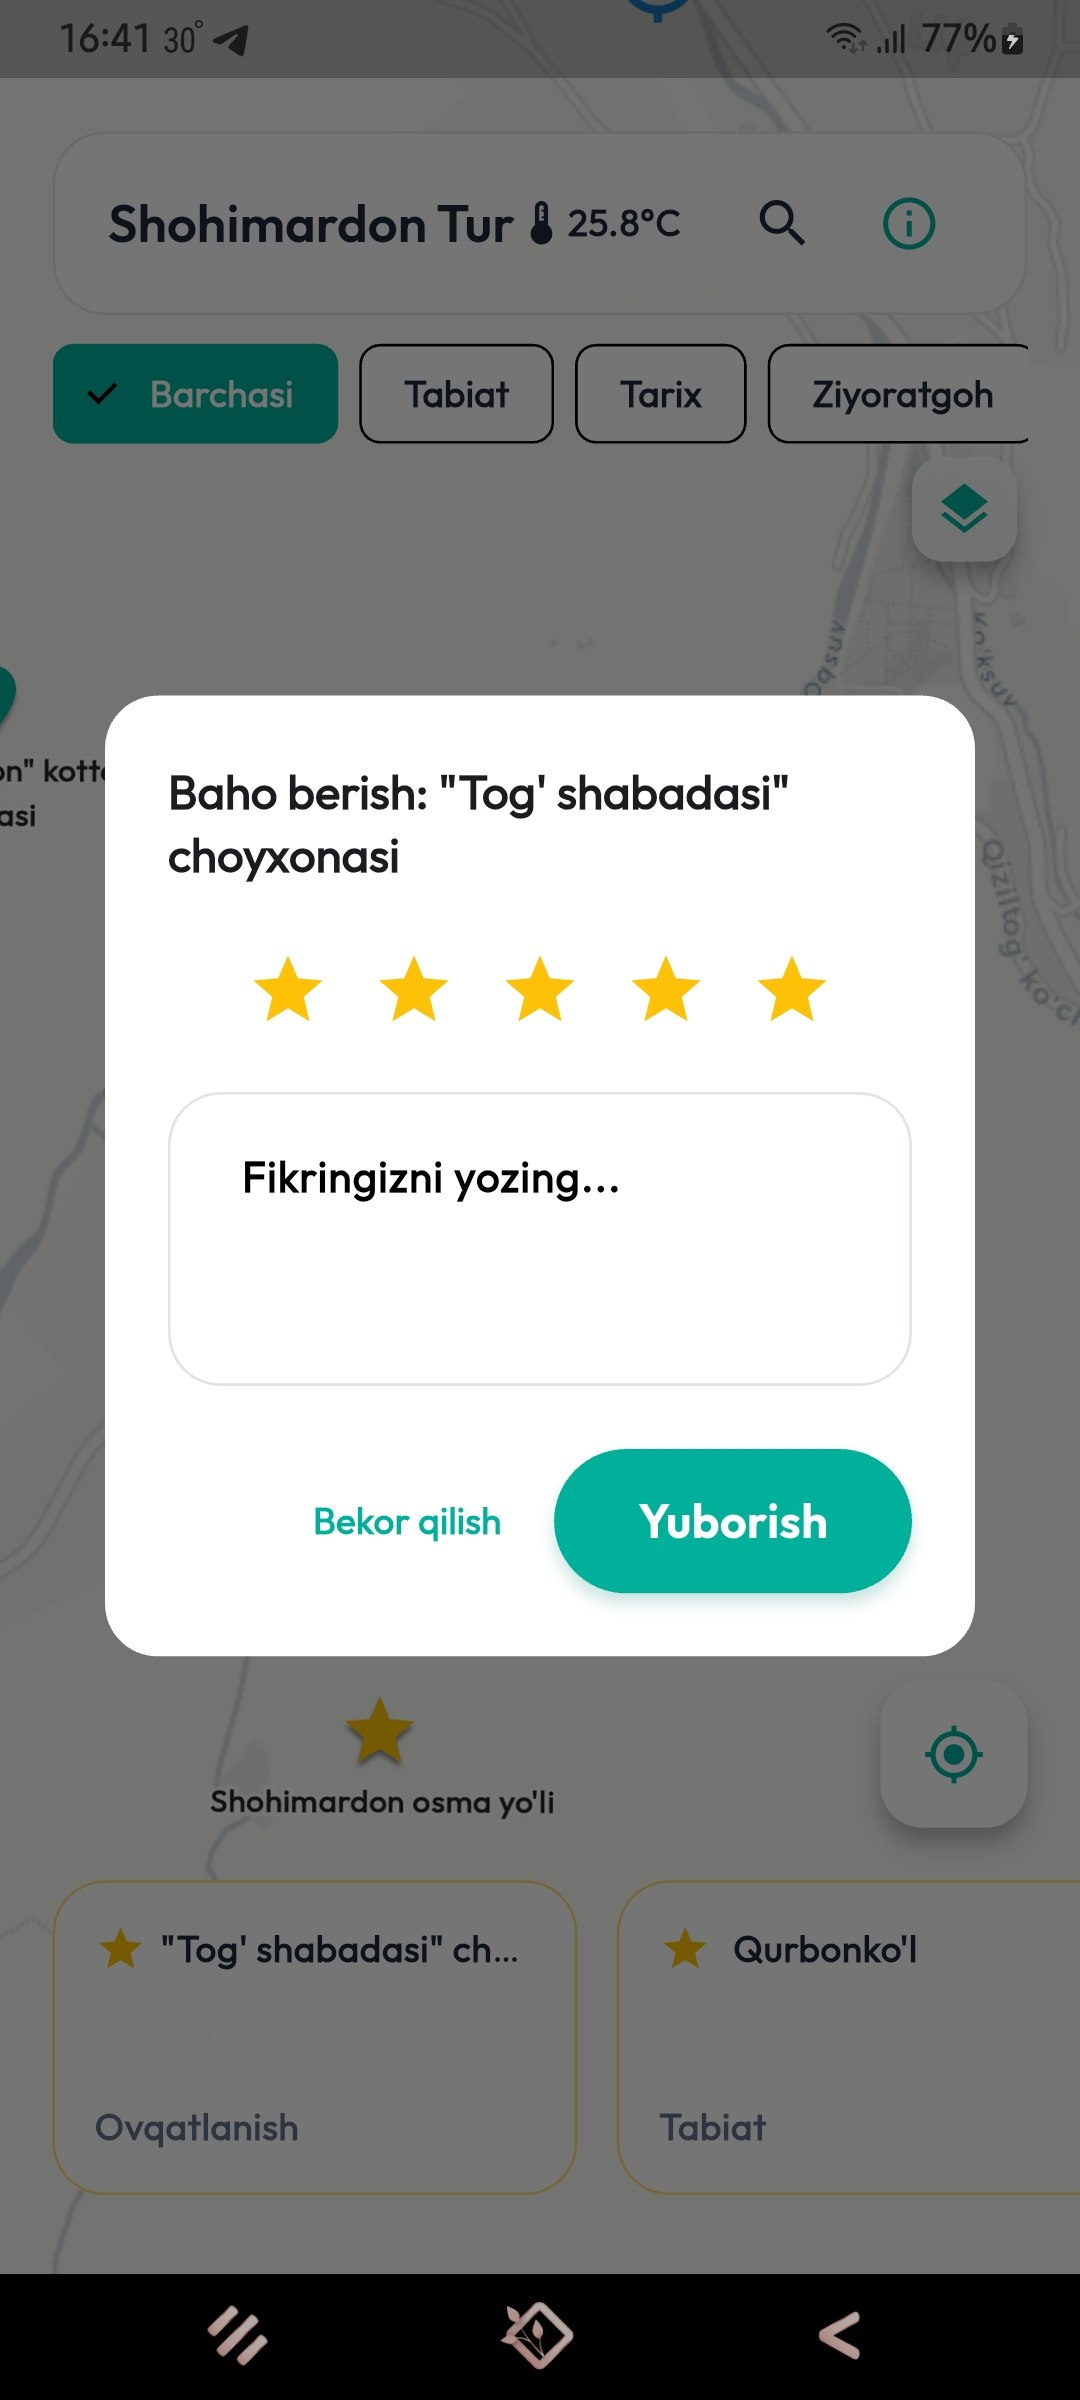
\includegraphics[height=5.6cm]{images/image16.png}\\[0.4cm]
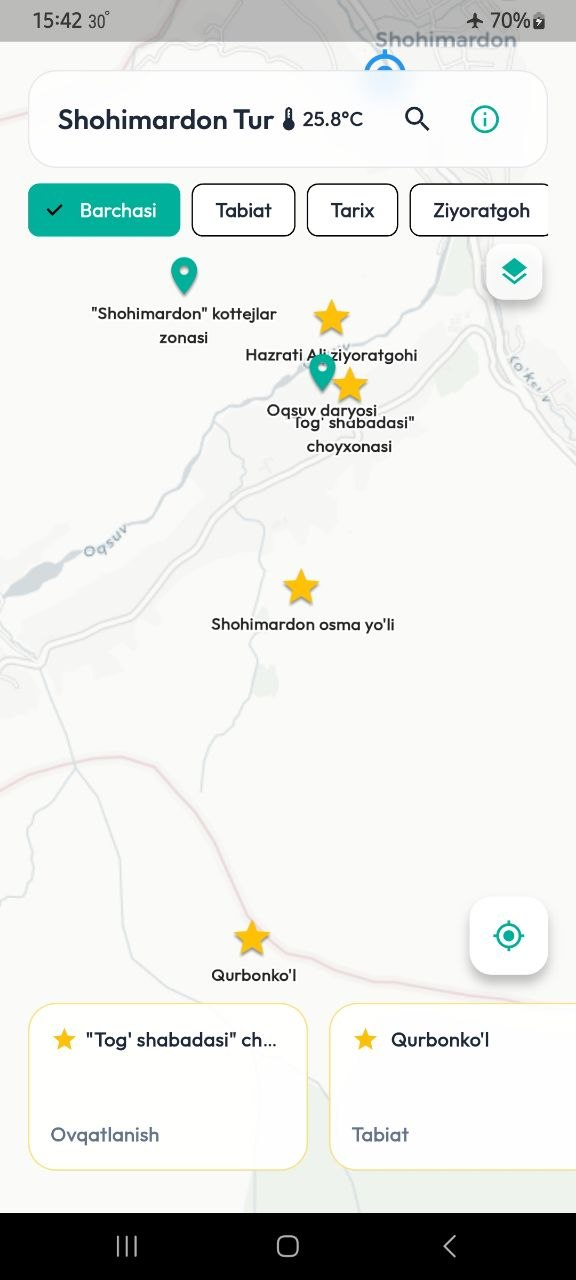
\includegraphics[height=5.6cm]{images/image13.png}\hfill
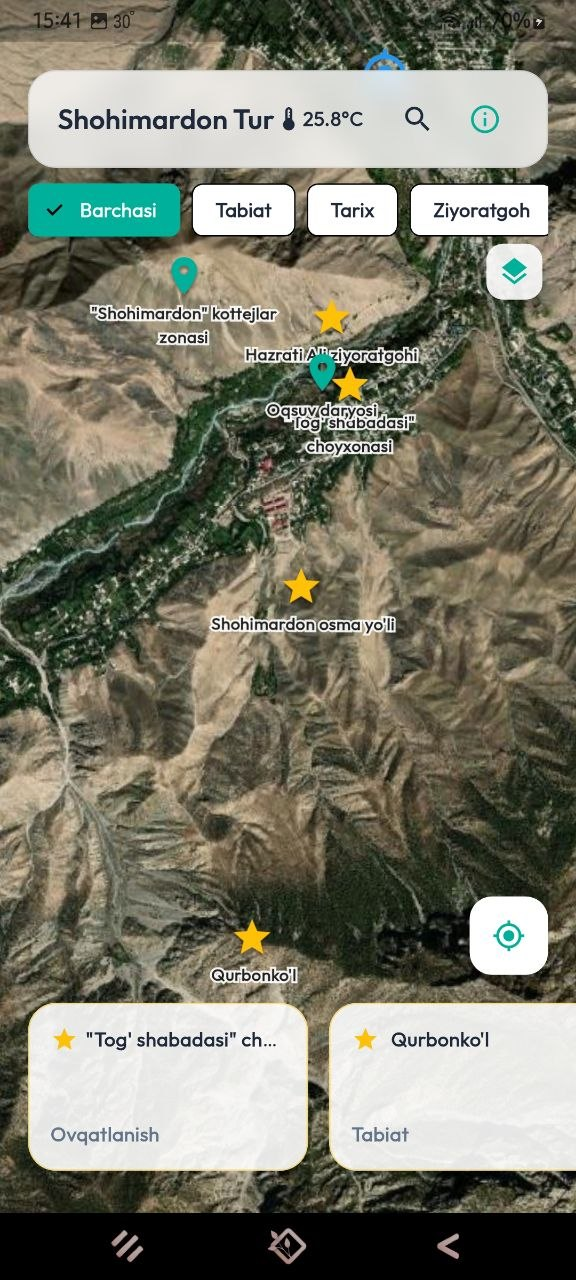
\includegraphics[height=5.6cm]{images/image14.png}\hfill
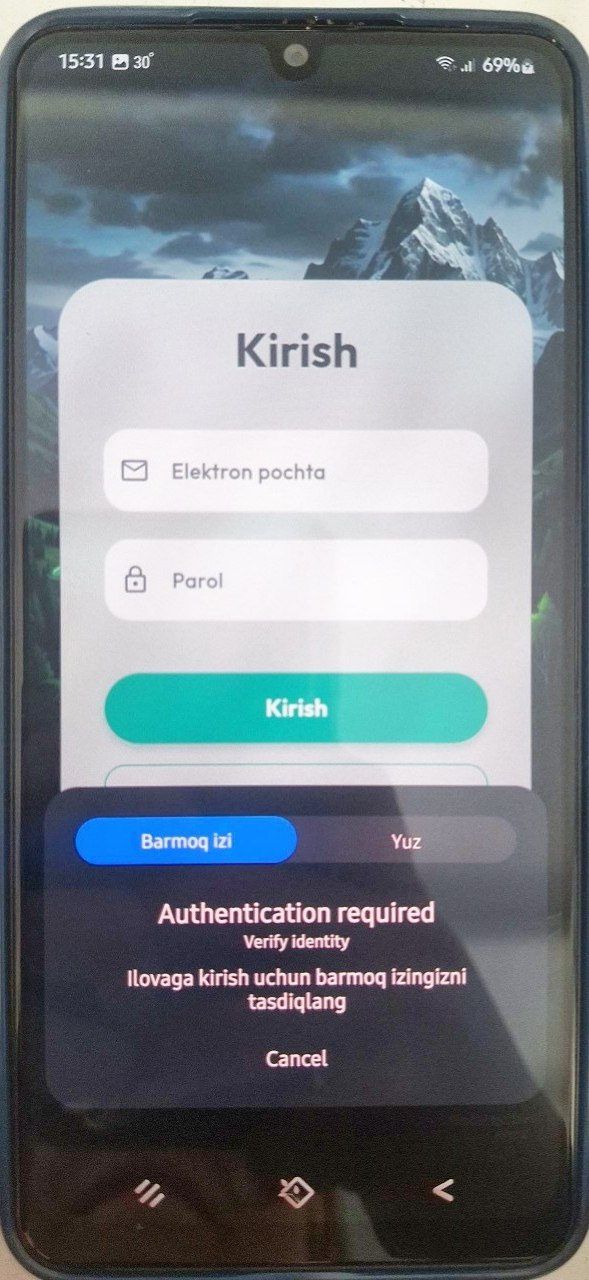
\includegraphics[height=5.6cm]{images/image15.png}
\caption{Compiled prototype interfaces: language selection, login, offline review dialog
(top row); street map view, satellite map view, and biometric authentication (bottom row).}
\label{fig:ui}
\end{figure}

%==============================================================================
\chapter{DISCUSSION AND PRODUCTION PERSPECTIVES}
%==============================================================================

\section{Practical Testing Results and Application Metrics}

The empirical analysis of the ``Shohimardon Tour Travel'' prototype yields critical
insights into the operational efficiency of offline-first software architectures. By
implementing the BLoC pattern as the structural backbone, the presentation layer was
completely isolated from heavy data input/output routines.

During simulated field trials involving deep network degradation and absolute
infrastructure failure, the application managed user interactions dynamically, bypassing
external network validation by routing queries directly through the local NoSQL storage
cache via specialized \texttt{Source.cache} optimization pathways. Quantitative metric
logging indicated that points-of-interest arrays, navigation paths, and embedded textual
blocks loaded inside a 50-millisecond execution window. This latency optimization completely
prevents the 20-second connection timeout loops that typically cause web-dependent apps to
freeze.

To precisely quantify the improvements, the core data access layers were benchmarked under
varying infrastructure stress profiles. In standard web-dependent pipelines operating under
mountain terrain shadowing and a 40\% packet loss rate, continuous web-gateway polling and
synchronous HTTP handshakes routinely fail, forcing the runtime into an extensive
20{,}000-millisecond network timeout penalty window. Conversely, the developed caching engine
operates under complete hardware isolation; by making a direct hardware I/O file read via
localized source-cache options, the lookup resolves as an instant cache hit within a
sub-50-millisecond window. Furthermore, by applying strict distance-change filtering and
high-precision accuracy filters, the location module successfully grouped multi-satellite
data layers, maintaining a highly accurate 3-to-5-meter tracking margin along unpaved
trekking paths without excessive CPU overhead or fast battery depletion.

\section{Importance of the App for Digitalization of Shohimardon Region Tourism}

Implementing an independent, offline-first mobile GIS is essential for bridging the digital
divide in topographically isolated regions like the Shohimardon enclave. Because of its
remote location and rugged alpine terrain, installing continuous high-speed cellular
networks is extremely difficult and expensive. Standard tourism applications rely heavily
on steady internet access, which leaves travelers vulnerable when navigating areas with
weak signals, unmapped trails, and minimal emergency connectivity.

Traditional tourism applications are fundamentally bound to continuous cloud-based
architectures, requiring a steady connection to external web-gateways to render map layers,
process spatial data, and handle database transactions. In contrast, the Shohimardon
prototype utilizes completely decoupled internal memory structures, relying on pre-packaged
static asset bundles and localized disk sandboxes compiled directly inside the client
device's physical partition, removing any requirement for live server pings. When entering
remote zones characterized by severe signal shadowing, traditional platforms immediately
drop active socket connections and throw unhandled runtime exceptions, whereas the developed
prototype remains fully operational even under absolute cellular failures, handling all
interactions through local processing paths and maintaining a stable frame rate.

This prototype overcomes connectivity barriers by embedding vector map assets, regional
business directories, and multi-lingual language arrays directly into the client device's
physical memory space. By making detailed local information accessible without cellular data
or expensive international roaming fees, the application strengthens the regional economy,
connecting travelers directly with small-scale homestays, local guides, and artisanal craft
shops, and establishing a scalable model for eco-tourism development across Uzbekistan.

\section{Technical Limitations and Hardware Issues of the Prototype}

While the prototype demonstrates high operational stability during field testing, it
exhibits several technical and structural constraints that must be addressed before moving
to full-scale production:

\begin{itemize}[leftmargin=1.4em]
  \item \textbf{Linear Binary Storage Footprint Growth:} because the application
        pre-packages pre-rendered raster map components, localized translation blocks, and
        media files within the core installation bundle, the app's size increases linearly
        as the targeted geographic boundaries expand, posing a deployment barrier on
        low-end smartphones.
  \item \textbf{Initial Cache Bootstrap Vulnerabilities (Cold Starts):} the synchronization
        architecture relies on an established data link during its first deployment phase to
        map out the master Firestore schemas. If a user first opens the app while already
        inside a dead zone, initialization fails.
  \item \textbf{Severe Physical GNSS Multipath Interference:} high rocky canyon walls and
        dense forest canopies introduce severe satellite signal reflections, causing
        unavoidable location jumping that client-side filters cannot entirely eliminate
        without secondary hardware sensors.
  \item \textbf{Battery Consumption Under Continuous Tracking:} maintaining the multi-GNSS
        chips at maximum high-precision levels rapidly accelerates battery consumption,
        making long-term continuous field tracking difficult without native background power
        throttling.
\end{itemize}

\section{Future Plans and Migration to Full Production System}

Transitioning the prototype into a scalable, enterprise-grade ecosystem requires refining
the data architecture, reducing memory overhead, and broadening community integrations. To
resolve the binary storage footprint constraints, the current pre-packaged map structure
will be replaced by an on-demand, server-driven vector tiling management system, allowing
users to selectively download compressed geographical packages while keeping the core
bundle lightweight. The database access layers will be upgraded with specialized
conflict-resolution models to manage multi-user review concurrency control, ensuring that
when thousands of tourists submit reviews offline, the background replication layer safely
reconciles the data streams upon reconnection.

To expand practical utility for the local population, the data structures will be linked
with a low-bandwidth Telegram bot system designed to share real-time navigation and queue
management updates for pharmacies across the Fergana region, addressing critical community
healthcare access needs alongside tourist navigation. Finally, native enhancements will
include integrating the smartphone's internal barometric sensors to calibrate altitude
readings, giving trekkers precise elevation metrics when navigating mountain passes.

%==============================================================================
\chapter*{GENERAL CONCLUSION}
\addcontentsline{toc}{chapter}{GENERAL CONCLUSION}
\markboth{GENERAL CONCLUSION}{}
%==============================================================================

The development and technical evaluation of the ``Shohimardon Tour Travel'' mobile
application prototype demonstrates the real-world viability of an offline-first
architectural paradigm for digitalizing regional tourism in topographically isolated
geographies. Traditional mobile tourism applications fail in harsh infrastructure conditions
because they rely on synchronous, network-blocking database connections. This project
addresses the digital divide by building an autonomous, decoupled navigation and information
framework directly into the client smartphone hardware. The core structural conclusions and
achievements are summarized below:

\begin{itemize}[leftmargin=1.4em]
  \item \textbf{Architectural Decoupling and State Stability:} implementing the BLoC state
        management pattern completely isolated the presentation layer from heavy I/O loops,
        preventing interface freezing and ensuring a fluid graphical interface at a stable
        60 to 120 FPS profile.
  \item \textbf{Data Access Optimization:} configuring the client-side Cloud Firestore SDK
        with local disk persistence and unlimited caching bypassed traditional timeouts,
        dropping document retrieval latency to under 50 milliseconds --- an exceptional
        optimization compared to the standard 20{,}000-millisecond timeout window of
        web-dependent software.
  \item \textbf{Linguistic and Spatial Autonomy:} a client-side multi-lingual engine using
        RAM-allocated static JSON dictionaries alongside nested NoSQL maps enabled
        instantaneous language switching under network isolation, while high-precision GNSS
        parameters stabilized tracking margins to 3-to-5 meters.
  \item \textbf{Mitigation of System Restrictions:} comprehensive simulation testing
        identified clear boundaries --- linear storage growth and cold-start vulnerabilities
        --- providing a concrete technical roadmap for production migration.
\end{itemize}

Ultimately, this graduation project proves that mobile tourism software can remain highly
reliable, performant, and safe without relying on a constant cellular internet connection.
By delivering secure base map layouts, offline regional business coordinates, and
multi-lingual descriptors directly from internal storage paths, the prototype provides an
actionable technological blueprint for rural digitalization. Expanding this data layer into
an on-demand vector tile management system and integrating it with local low-bandwidth
community networks will turn this prototype into a sustainable, community-wide enterprise
application.

%==============================================================================
\chapter*{REFERENCES}
\addcontentsline{toc}{chapter}{REFERENCES}
\markboth{REFERENCES}{}
%==============================================================================

\begin{enumerate}[leftmargin=2em,label={[\arabic*]}]
  \item Alishev, S., \& Karimov, T. (2024). \emph{Digitalization of Tourism Infrastructure
        in Mountainous Regions of Central Asia}. Tashkent: Fan nashriyoti.
  \item Bloc Library Authors. (2025). \emph{BLoC State Management Architecture Pattern for
        Cross-Platform Desktop and Mobile Applications}. Retrieved from
        \url{https://bloclibrary.dev/}
  \item Cloud Firestore Documentation Team. (2025). \emph{Configure Offline Data
        Persistence and Client-Side Cache Allocation Rules for NoSQL Collections}. Google
        Firebase Developer Core Documentation.
  \item Evans, R., \& Smith, J. (2023). \emph{Mobile GIS Architecture: Building
        Network-Isolated Navigation and Mapping Systems}. Academic Press.
  \item Flutter Engine Architecture. (2024). \emph{Internationalization (i18n) and Localized
        JSON Dictionary Packing Engines for Cross-Platform Frameworks}. Dynamic Runtime UI
        Documentation.
  \item Hillel, M. (2022). \emph{Offline-First Mobile Application Design: Data
        Synchronization and Local Storage Paradigms under Unstable Networks}. O'Reilly Media.
  \item Kosimov, A. A., \& Rahmonov, M. D. (2023). \emph{Analysis of Geopolitical Enclaves
        and Topographical Isolation Infrastructure Challenges in Fergana Valley Region}.
        Journal of Central Asian Studies, 14(2), 112--128.
  \item LatLng Dynamic Mapping Library for Dart. (2024). \emph{Geospatial Coordinate Matrix
        Conversions and Mathematical Geofencing Algorithms for Mobile Disconnected Client
        Devices}. Pub.dev Repository.
  \item NASA GNSS Systems Working Group. (2021). \emph{Multipath Reflection, Satellite
        Shadowing, and Coordinate Calibration Models in Rugged Canyon Terrains}. GPS
        Technical Review, 88(4), 210--225.
  \item Shodiyev, B. (2025). \emph{Developing Multi-lingual Systems and Local Asset Storage
        Matrices for Mobile Applications}. Tashkent State Technical University Academic
        Bulletin, 45--54.
  \item Tokhirov, F. (2024). \emph{The Impact of Digitalization Frameworks on Eco-Tourism
        and Local Hospitality Economies in Remote Areas of Uzbekistan}. Uzbekistan Economic
        Review, 19(3), 89--104.
  \item Wright, K. (2023). \emph{Optimistic Rendering and Conflict Resolution Queues in
        Asynchronous Database Synchronization Pipelines}. IEEE Transactions on Software
        Engineering, 49(7), 1432--1445.
\end{enumerate}

%==============================================================================
\appendix
\renewcommand{\thechapter}{\Alph{chapter}}
\titleformat{\chapter}[display]
  {\normalfont\Large\bfseries\color{rnublue}}
  {APPENDIX \thechapter}{12pt}{\LARGE}

\chapter{Static Interface Translation Dictionaries (JSON Asset Payloads)}
\addcontentsline{toc}{chapter}{APPENDIX A: Translation Dictionaries}

\textbf{1. English Dictionary File (\texttt{assets/lang/en.json})}
\begin{lstlisting}[language=]
{
  "app_title": "Shohimardon Tour Travel",
  "search_placeholder": "Search paths, landmarks...",
  "btn_navigate": "Start Route",
  "btn_language": "Change Language",
  "status_offline": "Running in Autonomous Offline Mode",
  "lbl_emergency": "Emergency Contacts"
}
\end{lstlisting}

\textbf{2. Uzbek Dictionary File (\texttt{assets/lang/uz.json})}
\begin{lstlisting}[language=]
{
  "app_title": "Shohimardon Tour Travel",
  "search_placeholder": "Yo'llar va qadamjolarni qidirish...",
  "btn_navigate": "Yo'nalishni boshlash",
  "btn_language": "Tilni o'zgartirish",
  "status_offline": "Avtonom oflayn rejimda ishlamoqda",
  "lbl_emergency": "Favqulodda aloqalar"
}
\end{lstlisting}

\chapter{Complete Multi-lingual Architecture and Localization Service Wrapper}
\addcontentsline{toc}{chapter}{APPENDIX B: Localization Service Wrapper}

\begin{lstlisting}[language=Dart]
import 'package:flutter/material.dart';
import 'package:flutter/services.dart';
import 'dart:convert';

class AppLocalizationService {
  final Locale locale;
  late Map<String, String> _localizedStrings;

  AppLocalizationService(this.locale);

  static AppLocalizationService? of(BuildContext context) {
    return Localizations.of<AppLocalizationService>(context, AppLocalizationService);
  }

  Future<bool> loadLocalizationAsset() async {
    try {
      String jsonString =
          await rootBundle.loadString('assets/lang/${locale.languageCode}.json');
      Map<String, dynamic> jsonMap = json.decode(jsonString);
      _localizedStrings = jsonMap.map((key, value) {
        return MapEntry(key, value.toString());
      });
      return true;
    } catch (exception) {
      _localizedStrings = {};
      return false;
    }
  }

  String translate(String key) {
    return _localizedStrings[key] ?? key;
  }

  static const LocalizationsDelegate<AppLocalizationService> delegate =
      _AppLocalizationDelegate();
}

class _AppLocalizationDelegate
    extends LocalizationsDelegate<AppLocalizationService> {
  const _AppLocalizationDelegate();

  @override
  bool isSupported(Locale locale) {
    return ['uz', 'en', 'ru'].contains(locale.languageCode);
  }

  @override
  Future<AppLocalizationService> load(Locale locale) async {
    AppLocalizationService localization = AppLocalizationService(locale);
    await localization.loadLocalizationAsset();
    return localization;
  }

  @override
  bool shouldReload(covariant LocalizationsDelegate<AppLocalizationService> old) => false;
}
\end{lstlisting}

\chapter{Core BLoC State Management Component Implementation}
\addcontentsline{toc}{chapter}{APPENDIX C: Core BLoC Component}

\begin{lstlisting}[language=Dart]
import 'package:flutter_bloc/flutter_bloc.dart';
import 'package:latlong2/latlong.dart';
import 'package:cloud_firestore/cloud_firestore.dart';

abstract class NavigationEvent {}
class InitializeNavigation extends NavigationEvent {}
class UpdateUserLocation extends NavigationEvent {
  final LatLng newLocation;
  UpdateUserLocation(this.newLocation);
}

abstract class NavigationState {}
class NavigationInitial extends NavigationState {}
class NavigationLoading extends NavigationState {}
class NavigationReady extends NavigationState {
  final LatLng userLocation;
  final List<DocumentSnapshot> cachedPlaces;
  final bool isOfflineMode;
  NavigationReady({
    required this.userLocation,
    required this.cachedPlaces,
    required this.isOfflineMode,
  });
}

class NavigationBloc extends Bloc<NavigationEvent, NavigationState> {
  final FirebaseFirestore _firestore = FirebaseFirestore.instance;

  NavigationBloc() : super(NavigationInitial()) {
    on<InitializeNavigation>(_onInitializeNavigation);
    on<UpdateUserLocation>(_onUpdateUserLocation);
  }

  Future<void> _onInitializeNavigation(
      InitializeNavigation event, Emitter<NavigationState> emit) async {
    emit(NavigationLoading());
    try {
      QuerySnapshot cacheQuery = await _firestore
          .collection('places')
          .get(const GetOptions(source: Source.cache));

      emit(NavigationReady(
        userLocation: const LatLng(39.9811, 71.8028),
        cachedPlaces: cacheQuery.docs,
        isOfflineMode: true,
      ));
    } catch (_) {
      emit(NavigationReady(
        userLocation: const LatLng(39.9811, 71.8028),
        cachedPlaces: const [],
        isOfflineMode: true,
      ));
    }
  }

  void _onUpdateUserLocation(
      UpdateUserLocation event, Emitter<NavigationState> emit) {
    if (state is NavigationReady) {
      final currentState = state as NavigationReady;
      emit(NavigationReady(
        userLocation: event.newLocation,
        cachedPlaces: currentState.cachedPlaces,
        isOfflineMode: currentState.isOfflineMode,
      ));
    }
  }
}
\end{lstlisting}

\end{document}
